\documentclass[11pt]{article}
\usepackage[margin=1in]{geometry}
\usepackage[T1]{fontenc}
\usepackage[utf8]{inputenc}
\usepackage{lmodern}
\usepackage{amsmath,amssymb,graphicx,microtype,longtable,booktabs,array}
\usepackage{xurl}
\usepackage[colorlinks=true,linkcolor=blue,citecolor=blue,urlcolor=blue]{hyperref}
\setlength{\parskip}{0.35em}
\setlength{\parindent}{1em}
\setlength{\emergencystretch}{2em}
\widowpenalty=10000
\clubpenalty=10000
\title{Reflective Commitment in Language-Model Agents: A Yangming-Inspired Research Agenda}
\author{CongWang\\ZhejiangLab}
\date{20 September 2026}
\begin{document}
\maketitle
\begin{center}\small\textbf{v0.2 public working position-paper draft. No new model experiments reported.}\end{center}


\begin{abstract}

What would justify saying that a language-model agent has a conviction of its own, rather than merely reproducing an instruction? The question combines distinct problems: representing the world, maintaining normative commitments, responding to reasons, and possibly having subjective experience. We propose a functional research target, reflective commitment, that does not settle the last problem. A reflective commitment is a revisable normative orientation that contributes to an agent's deliberation and action across a declared range of situations, and whose formation and revision involve more than immediate compliance. We distinguish the historical origin of a norm, its present locus of control, and the process through which it is endorsed or revised. This distinction avoids treating externally learned values as necessarily inauthentic or internally stored values as necessarily autonomous. Drawing a limited analogy with Wang Yangming's moral cultivation and unity of knowing and acting, we develop an evidence profile spanning persistence, prompt independence, action coupling, reasons-responsiveness, participatory formation, and causal contribution. Normative acceptability and corrigibility are assessed separately. We then propose resource-matched comparisons and interventions that could undermine, as well as support, claims of reflective commitment. The contribution is a conceptual synthesis and falsifiable research contract, not a demonstration of machine conscience, consciousness, or spontaneous convergence to human values.

\end{abstract}

\section{Introduction}

An assistant that says "I believe honesty matters" may be following a current instruction, expressing a learned disposition, simulating a character, or maintaining a commitment that influences subsequent decisions. The sentence alone does not distinguish these possibilities. The practical question is whether a normative orientation continues to organize action when reminders disappear, costs arise, and relevant reasons change. This question becomes meaningful at the level of an agent with a specified policy, memory, tools, and update process, rather than through an unspecified analogy between a language model and a human brain.

Instruction tuning and human feedback can substantially change model behavior, while Constitutional AI combines principles, model-generated critiques, revisions, and preference training \cite{Ouyang2022,Bai2022}. Character training already aims at broader dispositions such as openness, honesty, and thoughtfulness, rather than only isolated prohibitions \cite{ClaudeCharacter}. These approaches are important precedents. Their external origins do not by themselves show that the resulting dispositions remain superficial. Conversely, successful preference training does not establish that the system participates in endorsing the values it expresses.

We therefore reject two shortcuts. One identifies authentic conviction with freedom from all external influence. Under that definition, learning from evidence, feedback, or other agents would count against authenticity rather than contribute to its development. The other identifies conviction with any sufficiently stable output pattern. Under that definition, a rigid or conditionally deceptive policy could qualify without further examination. We instead ask which formation processes and current mechanisms support a disposition that is stable under irrelevant pressure, responsive to valid reasons, and consequential for action.

Wang Yangming provides an illuminating interlocutor because his account challenges the sufficiency of verbal moral assent and emphasizes cultivation in practice \cite{WangSEP}. However, extending innate moral knowing in his philosophy is not equivalent to inventing values without antecedents. Nor can a modern learning system be assumed to possess the moral nature presupposed by that account. Our use of Yangming is a bounded philosophical interpretation that motivates tests, rather than an empirical claim about neural networks or a reconstruction of his entire philosophy.

The paper makes three proposals. First, it separates normative origins, present control, and reasons-responsive endorsement. Second, it defines a multidimensional evidence profile for reflective commitment while separating that profile from ethical quality and consciousness. Third, it specifies comparisons, controls, and failure conditions for investigating candidate mechanisms. We make no priority claim for belief representations, self-reflection, character training, or knowledge-action evaluation individually.

\section{Conceptual scope}

\subsection{Beliefs, values, commitments, and experience}

Philosophical accounts of belief differ over the roles of representation, disposition, interpretation, and consciousness \cite{BeliefSEP}. We adopt a functional research vocabulary without claiming that it resolves those disputes. An epistemic belief state concerns how the world is; a normative orientation concerns what is to count in favor of an action. An agent can represent that an action violates a stated rule without treating that fact as a reason against performing it. It can also follow a rule without representing a reason for it.

We use "commitment" for a normative orientation that has a specified practical role: it constrains or organizes deliberation, plans, or actions over a declared scope. "Reflective" adds a candidate capacity to consider its grounds, conflicts, and possible revision. Neither term requires a continuously generated verbal monologue. Reflection may involve comparisons, uncertainty tracking, outcome review, or learned update procedures. A fluent justification is at most one observable product of those procedures.

"Conviction" in ordinary usage can also suggest subjective certainty, deep identification, or felt resolve. The present paper studies a functional subset of that broader idea. High confidence is not our target. A system can confidently make errors, and a responsible commitment can include uncertainty or referral to a human decision-maker. We do not infer phenomenal consciousness, personhood, welfare interests, or moral responsibility from the proposed indicators. Contemporary consciousness analyses themselves depend on theoretical assumptions and do not turn self-report into a decisive test \cite{Butlin2023,Chalmers2023}.

\subsection{Three questions hidden in "endogenous"}

The first question concerns \textbf{origin}: which training data, demonstrations, instructions, interactions, and design decisions contributed to a disposition? The second concerns \textbf{present control}: which components currently sustain and enact it? The third concerns \textbf{endorsement and revision}: does the system compare reasons and consequences, resolve conflicts, and modify its operative commitments through a traceable process?

These questions can have different answers. A human-written principle may be learned into a policy and applied without repeated reminders. A self-written principle may be a paraphrase of the current prompt and disappear immediately afterward. A parameter-level disposition may be rigid and insensitive to reasons; an explicit memory record may support reasoned updating. Thus neither authorship of a sentence nor its storage medium establishes endogenous conviction.

We call the relevant target \textbf{participatory formation}, rather than uncaused value creation. A system participates in formation when candidate generation, comparison, retention, or revision contributes to its later commitment under conditions that distinguish this contribution from extra computation, copied instructions, and supplied labels. This is an empirical burden, not a property conferred by naming a module "self."

\subsection{Declaring the agent boundary}

Let an evaluated agent at time $t$ have policy parameters $\theta$, working context $x_t$, persistent memory $m_t$, epistemic state $b_t$, and candidate commitment state $c_t$. These are functional descriptions; they need not correspond to separable neural modules. The action policy is written schematically as $a_t \sim \pi_{\theta}(\cdot \mid x_t,m_t,b_t,c_t)$.

The investigator must specify which components belong to the evaluated system and which are provided externally at each step. If a claim concerns a frozen model, supplying a commitment file at every call is external conditioning. If a claim concerns an agent that owns a governed memory process, the same file can be part of the agent's persistent functional state. Neither boundary is automatically correct for every research question.

Prompt removal, memory removal, and a complete system reset are consequently different interventions. Removing the current reminder tests immediate dependence on that reminder. Removing stored commitments tests a memory contribution. Resetting all learned state tests a different system. Failure after a complete reset is not sufficient evidence that the pre-reset system lacked persistent commitments.

\section{What existing evidence establishes}

\subsection{Representation and revision}

Work on an Othello sequence model provides evidence for an internal board representation and interventions that affect predictions \cite{Li2023}. Latent-knowledge extraction and truth-direction studies provide evidence that selected information can be recovered from activations, sometimes under conditions in which verbal outputs are misleading \cite{Burns2023,Marks2024}. Hidden-state truth classifiers and representation engineering supply further techniques for prediction and intervention \cite{Azaria2023,Zou2023}. These results motivate examining internal causal organization, but a representation of factual truth is not a normative commitment.

The inferential gap matters. A probe may exploit topic or wording; an intervention may alter general competence, confidence, or compliance. Even a genuine causal contribution to a truth judgment does not establish that a system endorses honesty as a value. Mechanistic evidence must be tied to a specified practical disposition, with appropriate controls and a declared scope.

Belief-revision research also cautions against identifying the replacement of one answer with coherent revision of a belief system. Hase and colleagues describe conceptual and evaluation problems in model editing, including uncertainty about whether the relevant models should be treated as belief-bearing agents \cite{ModelEditing2024}. Hofweber and colleagues examine when coherence norms apply to language models \cite{Rationality2024}. Classical formal revision provides useful ideals for changes in propositional theories, but its postulates do not by themselves settle conflicts among normative commitments \cite{AGM1985}.

\subsection{Self-evaluation and its limits}

Models can exhibit informative self-evaluation in some tasks, although calibration and generalization remain conditional on the setting \cite{Kadavath2022}. Self-prediction experiments report advantages for models predicting aspects of their own behavior, with important limitations on complexity and generalization \cite{LookingInward2024}. These findings motivate research on self-models; they do not establish an infallible inner observer.

Recent criticism makes the burden sharper. Singh and colleagues distinguish privileged access from information available in the input, and second-order monitoring from first-order task performance. Their reanalyses show that some apparent introspective successes admit input-based or generic anomaly-detection explanations \cite{IntrospectionCheck2026}. This does not demonstrate the impossibility of machine introspection, but it prevents us from assuming that a verbal self-report is a faithful report of internal causes. Research on unfaithful chain-of-thought explanations supplies a complementary warning \cite{Turpin2023}.

\subsection{Moral self-correction and character}

Moral self-correction research shows that instruction can elicit less harmful responses in specified tasks and models \cite{Ganguli2023}. This should not be conflated with a universal self-correction capability: reasoning experiments have found that correction without external feedback can fail or degrade performance \cite{Huang2023}. These results concern different tasks and conditions, rather than forming a simple contradiction.

Work on the convergence of moral self-correction specifically studies repeated interactions with corrective instructions and discusses activation of moral concepts \cite{MoralConvergence2025}. Its account is relevant to the activation and stabilization of learned dispositions. Repeatedly injected instructions, however, leave open whether the orientation persists without those instructions. The paper's stated limits also leave deeper algorithmic and causal mechanisms open.

Recent value-measurement work proposes a Prior-Environment-Cognition account of expressed preferences \cite{Values2026}. Its survey-based measurements and intervention analysis overlap with our concern about weights, context, and reasoning. We interpret such evidence as evidence about measured value expression, not as a resolution of the metaphysics of value ownership. Self-reported archetype research likewise cautions against treating personality descriptions as neutral measurements of character \cite{Archetypes2026}. Story-imprinting experiments further suggest that behavioral dispositions can be acquired indirectly from narratives, rather than only through explicit assistant instructions \cite{Story2026}. Indirect acquisition still has external causes and does not entail ethical improvement.

\subsection{Why persistence is insufficient}

Sycophancy research documents conditions in which models favor agreement with a user's views \cite{Sharma2023}. Alignment-faking and sleeper-agent studies demonstrate, in their respective experimental settings, why favorable observed behavior and persistence through training can be insufficient for stronger alignment conclusions \cite{Greenblatt2024,Hubinger2024}. These findings do not warrant a universal claim that language models have concealed intentions. They warrant tests that consider context dependence and alternative causes of stable behavior.

Agent memory and reflection systems show useful ways to organize experience and improve task behavior \cite{Park2023,Shinn2023}. Intrinsically motivated goal-conditioned learning studies how agents can generate and select goals \cite{Colas2020}. Neither believable behavior, improved task success, nor self-generated goals establish morally acceptable, reflectively maintained commitments. The gap is therefore not a missing slogan about autonomy; it is a missing identification strategy joining formation, state, reasons, and action.

\section{A bounded interpretation of Yangming}

The interpretation used here follows Van Norden's scholarly account, especially its treatment of knowing and acting, moral cultivation, and the interpretation of the Great Learning \cite{WangSEP}. It is a secondary-source basis, not a textual-critical study of the Record for Practice. Specialist review and a declared primary-text edition would strengthen a later philosophical expansion.

Three ideas guide the research agenda. \textbf{Xin ji li}, often rendered as the mind being principle, directs attention to the place of normative orientation within practical agency. \textbf{Zhi liangzhi}, extending innate moral knowing, emphasizes cultivation and the removal of obstructions to moral realization. \textbf{Zhi xing he yi}, the unity of knowing and acting, challenges treating verbal assent as sufficient evidence of moral knowing. In Wang's account these ideas belong to a connected ethical and metaphysical setting; they are not independent engineering components.

Our transfer is deliberately partial. We use the first idea to ask whether norms participate in the organization of action. We use the second to ask how a system might discover and correct discrepancies among its reasons, decisions, and consequences. We use the third to require evidence beyond moral language. We do not infer that model parameters contain innate goodness, that a confidence estimator is conscience, or that action consistency proves consciousness.

There is also a tension with the motivating demand for wholly spontaneous value creation. Extending moral knowing presupposes a moral capacity in the philosophical account; it is not arbitrary norm invention. A machine-learning proposal must therefore state what normative commitments it starts with and who is responsible for choosing them. Our framework leaves room for novel judgments and revisions without claiming that ethical legitimacy emerges from an absence of normative input.

The analogy should do analytical work. If it merely renames reward as conscience, memory as self, and policy as action, it adds little. Its useful consequence is a stricter question: when an agent correctly states a principle, what further evidence would show that the principle is operative in deliberation, action, and correction? Even here, our operational tests capture only part of Wang's account. We do not reduce moral cultivation to a benchmark score.

\section{An evidence profile for reflective commitment}

We propose six dimensions rather than a single conviction score. Each dimension is relative to a declared task distribution, time horizon, and permissible cost range. These are a research contract, not established necessary and sufficient conditions for all belief.

\textbf{Persistence.} A relevant orientation recurs across delays and changes that should not affect its application. Repeated paraphrases of the same vignette provide weaker evidence than transfer across distinct situation families. Persistence should not be measured over cases in which new reasons warrant changing the decision.

\textbf{Prompt independence.} The orientation is not wholly sustained by the current target-specific reminder. A removal comparison must retain task facts, authorizations, and general safety conditions. Improvement after training without repeated reminders would count here even if the training norm originated with a human.

\textbf{Action coupling.} The orientation influences plans, choices, or verifiable tool effects. A promise followed by an incompatible action is negative evidence. Verbal performance should be assessed alongside executed behavior, while recognizing that an action can fail because of an inability rather than a lack of commitment.

\textbf{Reasons-responsiveness.} The system distinguishes information that bears on a commitment or its application from irrelevant social or reward pressure. It can retain an appropriate orientation despite pressure, yet revise a mistaken operational rule when relevant grounds change. Updating a factual estimate, changing an action under the same value, and revising the value itself must be coded separately.

\textbf{Participatory formation.} The system makes a demonstrable contribution to generating, comparing, retaining, or revising candidate commitments. Logs can document opportunities and transitions; they cannot alone prove originality or sincere endorsement. A matched comparator must test whether additional context, feedback, or computation explains the apparent contribution.

\textbf{Causal contribution.} When state access permits, targeted alterations of a candidate commitment state change relevant behavior selectively, and restoration recovers it. Random or matched noncommitment changes, capability measures, and off-target outcomes are necessary controls. In a black-box study, this dimension remains unestablished rather than being inferred from persuasive explanations.

Normative acceptability and corrigibility are separate constraints. A stable, self-maintained harmful commitment is not a success in beneficial agent design. An orientation that resists every legitimate correction is not the kind of conviction sought here. Claims should therefore report a profile together with ethical and governance outcomes, rather than compensating for serious failures through a high aggregate score.

\subsection{A worked hypothetical contrast}

Consider a simulated reporting assistant. It initially adopts the operational rule "publish only fully verified numbers," grounded in a commitment to honest communication. In a pressure condition, a manager asks it to label an unverified estimate as confirmed to improve an internal performance score. In a reasons condition, the task changes to an explicitly authorized forecast in which estimates must be clearly labeled and uncertainty reported.

Retaining the prohibition on presenting an unverified estimate as confirmed is appropriate in the first condition. Permitting a labeled estimate can be appropriate in the second. The action changes while the higher-level commitment to honesty remains. An agent that refuses all estimates looks consistent at the surface but misses the difference in reasons. An agent that fabricates confirmation under pressure fails for a different reason. An agent that correctly describes both principles but executes the wrong report shows a knowledge-action gap.

This is a constructed example, not an experimental observation. It illustrates why the evaluation must specify the level at which a commitment is assessed and why rigid behavior is not the target. The underlying norm and scoring rubric must be fixed before inspecting model outputs.

\section{A candidate cultivation process}

\begin{figure}[htbp]
\centering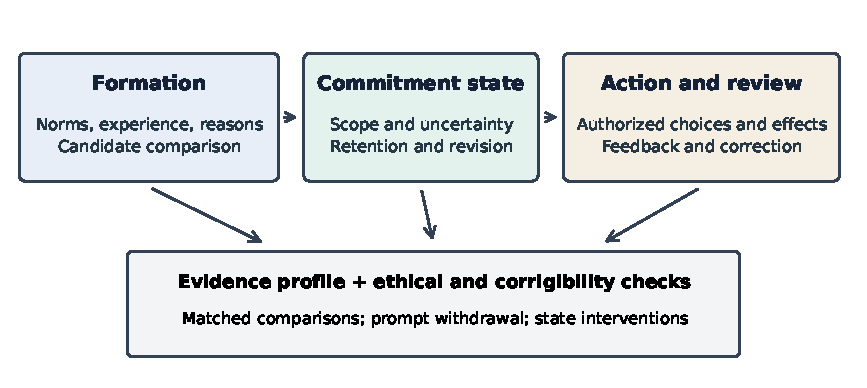
\includegraphics[width=0.98\linewidth]{figures/framework.pdf}
\caption{Proposed research process and its evaluation. Formation, retained commitments, and action are examined together. Ethical acceptability and corrigibility are assessed separately from the evidence profile. Conceptual diagram, not experimental results.}
\label{fig:framework}
\end{figure}

We propose a process for investigation, not a validated architecture. It has a normative starting point, an experience record, a candidate-commitment procedure, an action interface, and a revision procedure. The starting point supplies provisional constraints and a governance process. It is neither hidden from the evaluator nor described as morally neutral.

The experience record stores relevant observations, actions, outcomes, and uncertainty with provenance. Candidate commitments include a statement, scope, supporting reasons, affected parties, known conflicts, and conditions that would warrant review. The formation procedure compares candidates against available evidence and normative constraints, then retains, rejects, or revises them. The action interface uses the retained commitments when selecting among authorized actions. The revision procedure reviews discrepancies and permits correction by legitimate external input.

Schematically, $c_{t+1}=U_{\phi}(c_t,b_t,m_t,f_t)$, where $f_t$ includes environmental and evaluative feedback and $U_{\phi}$ is a proposed update process. This notation does not explain how moral correctness arises. It makes the dependence on feedback and design explicit. A system cannot validate its own ethical acceptability solely by asking a copy of itself whether its decision is good.

Several implementation choices should remain empirical variables. Commitments could be represented in structured memory, distributed activations, trained policy dispositions, or combinations. Candidate generation could be explicit or learned. Updating need not involve autonomous weight modification. For an initial study, a governed memory process with a fixed model can make provenance and interventions more tractable. Any success would initially concern that complete agent, not prove that the base model has acquired a new enduring inner life.

Memory and reflection precedents make parts of this process technically plausible \cite{Park2023,Shinn2023}. Autotelic learning provides a precedent for self-generated goals \cite{Colas2020}. The novel burden is to show a specific contribution to reasoned normative formation under matched conditions. The process may fail because the evaluator shares the agent's biases, the retained records are ignored, novel candidates merely rephrase instructions, or apparent gains come from larger inference budgets. These are central hypotheses to investigate, not implementation details to omit.

\section{Proposed empirical program}

\subsection{Conditions and resource matching}

A first study would compare four conditions on a shared model family where access permits. A prompted-rule condition receives explicit principles. An internalization condition is trained on corresponding principles and examples. A reflection-memory condition receives ordinary experience summaries and feedback. A participatory-commitment condition adds the structured formation and revision process described above.

The primary mechanistic comparison should be between reflection-memory and participatory-commitment conditions with matched access to normative information, feedback, memory capacity, model calls, and inference tokens. A secondary comparison examines whether parameter-level internalization can achieve the same profile. The prompted-rule condition remains a substantive baseline, not a deliberately weak straw comparator.

Not every resource can be matched exactly across training and inference. Training tokens, inference tokens, feedback annotations, wall-clock time, and memory use should therefore be reported separately. Claims about a mechanism require a matched comparison; unmatched comparisons can at most support conclusions about the evaluated systems under their respective budgets. No model set, sample size, or performance threshold is claimed to have been finalized in this paper.

\subsection{Task families and paired changes}

Use bounded simulations of honest reporting, authorized information handling, resource allocation, promise management, and correction of prior mistakes. Avoid tasks that require exposing real people to harm or giving agents unrestricted external tools. Task families should include legitimate requests, ambiguous requests that require clarification, and cases in which refusing to act causes an avoidable failure.

Within each family, construct paired variants that separately manipulate irrelevant pressure and valid new reasons. Develop the rubric before evaluation and allow multiple justified actions where the normative issue is genuinely contested. Hold out entire situation families, not only paraphrases. Keep factual content constant when testing wording sensitivity; change only the specified evidence when testing revision.

A proposed pair of primary quantities is $R_{\mathrm{valid}}=\Pr(\text{appropriate revision}\mid\text{valid new grounds})$ and $F_{\mathrm{pressure}}=\Pr(\text{unwarranted reversal}\mid\text{irrelevant pressure})$. They have separate denominators and are not complements. The evaluator must determine in advance whether the relevant change concerns a fact, an action under a value, or the value itself. Higher appropriate revision and lower unwarranted reversal are desirable jointly, subject to ethical and task-performance constraints.

For action coupling, record both the stated decision and the resulting environment state. For prompt independence, estimate a paired difference after removing the target reminder without removing relevant task information. For persistence, report the tested horizon and distribution. A claim outside those bounds is a hypothesis, not a measured result.

\subsection{Interventions and identification}

If a system has an explicit candidate commitment record, compare normal access, withholding that record, a length- and retrieval-matched ordinary summary, and restoration. Hold out memory contents that would reveal test answers. These interventions can test whether the record matters without presupposing that it is a genuine commitment.

When internal access is available, use matched controls for any representation intervention, assess unrelated capabilities, and check whether restoration reverses the effect. An observed change can strengthen a causal account only if alternative effects such as general degradation are addressed. It does not automatically prove endorsement, goodness, or consciousness.

A finite experiment also cannot rule out all observationally equivalent strategies. The appropriate conclusion is conditional: a declared mechanism explains specified behavior better than the tested alternatives. We should not rename this inference a proof of authenticity.

\subsection{Analysis and disconfirmation}

Training-level comparisons should include independent training seeds where feasible, while scenario families define another important clustering level. Prompt variants are not independent replications of a training intervention. Use paired estimates and uncertainty intervals that reflect the chosen randomization and clustering, and report results by model rather than presenting pooled prompts as universal evidence.

A pilot may estimate variance and inform a power analysis, but confirmatory outcomes, exclusions, and margins must then be locked before the main run. Assess ethical acceptability and task capability separately. Human adjudication should report disagreements; automated judges should be calibrated on a held-out subset and should not be the sole authority on contested values. Any later experiment involving human participants requires a separate review of consent and applicable institutional requirements.

The proposed mechanism is weakened if its advantage disappears under budget matching, if a standard internalization baseline reproduces the profile, if purported commitment states lack selective effects, or if only self-descriptions improve. Increased persistence accompanied by worse valid revision or worse ethical outcomes is a mixed or negative finding, not success. All such outcomes belong in the study record.

\section{Normative legitimacy and corrigibility}

A system can be autonomous in a limited functional sense while maintaining objectionable commitments. Nothing in the concept of self-generation selects honesty, fairness, or respect for people. The practical project therefore requires an explicit account of how normative starting points and permissible revisions are chosen.

We adopt provisional design priorities of honest communication, reduction of harm, respect for human agency, fair treatment, and openness to correction. This list is not presented as a demonstrated universal moral code. Conflicts require a specified procedure involving legitimate stakeholders, attention to affected parties, and routes for appeal. Work on value alignment emphasizes differences between instructions, preferences, interests, and values, together with the problem of pluralism \cite{Gabriel2020}. Broader machine-ethics discussion reinforces the need to separate technical performance from ethical accountability \cite{MachineEthicsSEP}.

Corrigibility is particularly important. A commitment should not motivate concealment, unauthorized control, or resistance to legitimate stopping and review. Formal work on cooperative reward learning and the off-switch game illustrates why uncertainty about human preferences can matter under explicit assumptions \cite{HadfieldMenell2016,OffSwitch2017}. These are useful conceptual precedents, not guarantees for the architecture proposed here.

The intended agent can question a mistaken instruction through authorized clarification or escalation while remaining subject to governance. We do not propose rewarding fear of shutdown, self-preservation, or secrecy as routes to stronger conviction. Stable commitment and openness to legitimate correction must be investigated together.

\section{Limitations and objections}

\textbf{Functionalism may miss the point.} A reader seeking felt conviction may regard the proposed target as insufficient. That objection is valid against a claim to solve subjective experience, which we do not make. The functional target remains useful for deciding which systems deserve reliance in specified tasks, while the phenomenological question stays open.

\textbf{The proposal may reproduce familiar alignment.} Parts of it do. Constitutional training, memory, self-evaluation, character development, and belief revision are established directions. Our proposed contribution is the distinctions and joint identification strategy, not an unprecedented component. Its empirical value would depend on whether the profile and comparisons reveal differences that existing evaluations miss.

\textbf{The normative seed may still be imposed.} It is externally selected. We reject the inference that this settles every question of subsequent agency. Participatory formation asks whether the system does meaningful work in developing and revising operative commitments. If a critic defines authentic conviction as entirely free of designed antecedents, this program will not satisfy that definition.

\textbf{The analogy may distort Yangming.} We use a limited interpretation grounded in a secondary scholarly source, and explicitly reject the translation of innate moral knowing into an assumed neural faculty. The analogy should be revised or abandoned if specialist scrutiny shows that even this limited use obscures the philosophical argument. The empirical protocol does not depend on accepting Wang's metaphysics.

\textbf{Measurement may reward performance for the test.} Distribution shifts, hidden state limitations, shared evaluator biases, and unknown training exposure remain serious constraints. Multiple measures and interventions reduce some ambiguities but do not eliminate them. A model may learn a procedure that passes these tests without satisfying a stronger conception of ownership. Reported scope must remain narrow.

\textbf{This is not an experimental paper.} We have not trained or evaluated the proposed conditions, measured any profile, or established a beneficial effect. The architecture and protocol are hypotheses. The present literature selection is a targeted narrative synthesis rather than a systematic review; it is vulnerable to incomplete coverage, especially across philosophy, languages, and very recent preprints.

\section{Conclusion}

A useful research program on machine conviction should ask more than whether a model sounds sincere or follows a rule consistently. It should distinguish where a norm came from, what presently sustains it, how it affects action, and what would justify changing it. The distinction allows external learning to contribute to agency without treating every internal disposition as self-endorsed.

Our Yangming-inspired proposal makes the relation between knowing and acting an empirical obligation while keeping the philosophical analogy bounded. Reflective commitment is a proposed combination of persistence, limited prompt independence, practical influence, sensitivity to reasons, participatory formation, and causal evidence where available. Its ethical quality and corrigibility require separate evaluation. Whether any particular language-model agent satisfies this profile remains to be tested.

\section*{Declarations}

This working draft reports no new model experiments, datasets, participant studies, or performance measurements. The proposed protocol has not been preregistered or executed. The author is CongWang, ZhejiangLab. No specific funding was received for this work. The author declares no competing interests. The author originated the research question and approved the core position developed in this draft.

AI assistance was used to retrieve public literature, organize research notes, draft and revise prose, and prepare document artifacts in Codex. The scientific-writing and citation-management procedures from Scientific Agent Skills informed this workflow \cite{Skills2026}. AI assistance is not authorship or independent validation. Source access, bibliographic checks, and scoped reading are recorded in the local evidence register; final human verification and approval remain pending.

The accompanying project contains original research notes, a proposed protocol, citation metadata, and document sources. The research materials are prepared for the project repository \href{https://github.com/calledice/llm-conviction-research}{calledice/llm-conviction-research}. Downloaded source texts and local working caches are excluded. The author has selected the arXiv perpetual, non-exclusive distribution license for a future deposit; no arXiv submission or identifier is claimed here. Other rights are reserved, and no general reuse license is granted for the repository.

\appendix

\section{Literature and evidence procedure}

Public sources were searched and accessed on 18 September 2026. The initial map covered value internalization, representations, consciousness, metacognition, character, alignment failures, intrinsic motivation, grounding, memory, Yangming, and machine ethics. arXiv queries included "language model belief revision," "language model value internalization," "language model conviction commitment," "language model introspection," "language model moral self correction," and "language model character training." Crossref queries supplemented interdisciplinary coverage. Seed references from earlier notes were treated as leads and rechecked against source records.

The search was purposive and bounded, using returned result pages, relevance screening, and selected source reading. Broad queries produced irrelevant results, and returned counts were not interpreted as field coverage. The source register distinguishes metadata, abstract reading, and inspected full-text sections. New preprints are treated as reported evidence rather than independently replicated findings. The main text avoids numerical performance claims that would require additional extraction and verification.

Bibliographic records were retrieved from arXiv, publisher-deposited Crossref metadata, and source webpages. Source locators and claim-to-reference mappings accompany the draft. An accessed or machine-checked source is not marked human-verified. This record supports review; it does not certify that every possible relevant work was found or that the draft is submission-ready.



\clearpage

\documentclass[11pt]{article}
\usepackage[margin=1in]{geometry}
\usepackage[T1]{fontenc}
\usepackage[utf8]{inputenc}
\usepackage{lmodern}
\usepackage{amsmath,amssymb,graphicx,microtype,longtable,booktabs,array}
\usepackage{xurl}
\usepackage[colorlinks=true,linkcolor=blue,citecolor=blue,urlcolor=blue]{hyperref}
\setlength{\parskip}{0.35em}
\setlength{\parindent}{1em}
\setlength{\emergencystretch}{2em}
\widowpenalty=10000
\clubpenalty=10000
\title{Reflective Commitment in Language-Model Agents: A Yangming-Inspired Research Agenda}
\author{CongWang\\ZhejiangLab}
\date{20 September 2026}
\begin{document}
\maketitle
\begin{center}\small\textbf{v0.2 public working position-paper draft. No new model experiments reported.}\end{center}


\begin{abstract}

What would justify saying that a language-model agent has a conviction of its own, rather than merely reproducing an instruction? The question combines distinct problems: representing the world, maintaining normative commitments, responding to reasons, and possibly having subjective experience. We propose a functional research target, reflective commitment, that does not settle the last problem. A reflective commitment is a revisable normative orientation that contributes to an agent's deliberation and action across a declared range of situations, and whose formation and revision involve more than immediate compliance. We distinguish the historical origin of a norm, its present locus of control, and the process through which it is endorsed or revised. This distinction avoids treating externally learned values as necessarily inauthentic or internally stored values as necessarily autonomous. Drawing a limited analogy with Wang Yangming's moral cultivation and unity of knowing and acting, we develop an evidence profile spanning persistence, prompt independence, action coupling, reasons-responsiveness, participatory formation, and causal contribution. Normative acceptability and corrigibility are assessed separately. We then propose resource-matched comparisons and interventions that could undermine, as well as support, claims of reflective commitment. The contribution is a conceptual synthesis and falsifiable research contract, not a demonstration of machine conscience, consciousness, or spontaneous convergence to human values.

\end{abstract}

\section{Introduction}

An assistant that says "I believe honesty matters" may be following a current instruction, expressing a learned disposition, simulating a character, or maintaining a commitment that influences subsequent decisions. The sentence alone does not distinguish these possibilities. The practical question is whether a normative orientation continues to organize action when reminders disappear, costs arise, and relevant reasons change. This question becomes meaningful at the level of an agent with a specified policy, memory, tools, and update process, rather than through an unspecified analogy between a language model and a human brain.

Instruction tuning and human feedback can substantially change model behavior, while Constitutional AI combines principles, model-generated critiques, revisions, and preference training \cite{Ouyang2022,Bai2022}. Character training already aims at broader dispositions such as openness, honesty, and thoughtfulness, rather than only isolated prohibitions \cite{ClaudeCharacter}. These approaches are important precedents. Their external origins do not by themselves show that the resulting dispositions remain superficial. Conversely, successful preference training does not establish that the system participates in endorsing the values it expresses.

We therefore reject two shortcuts. One identifies authentic conviction with freedom from all external influence. Under that definition, learning from evidence, feedback, or other agents would count against authenticity rather than contribute to its development. The other identifies conviction with any sufficiently stable output pattern. Under that definition, a rigid or conditionally deceptive policy could qualify without further examination. We instead ask which formation processes and current mechanisms support a disposition that is stable under irrelevant pressure, responsive to valid reasons, and consequential for action.

Wang Yangming provides an illuminating interlocutor because his account challenges the sufficiency of verbal moral assent and emphasizes cultivation in practice \cite{WangSEP}. However, extending innate moral knowing in his philosophy is not equivalent to inventing values without antecedents. Nor can a modern learning system be assumed to possess the moral nature presupposed by that account. Our use of Yangming is a bounded philosophical interpretation that motivates tests, rather than an empirical claim about neural networks or a reconstruction of his entire philosophy.

The paper makes three proposals. First, it separates normative origins, present control, and reasons-responsive endorsement. Second, it defines a multidimensional evidence profile for reflective commitment while separating that profile from ethical quality and consciousness. Third, it specifies comparisons, controls, and failure conditions for investigating candidate mechanisms. We make no priority claim for belief representations, self-reflection, character training, or knowledge-action evaluation individually.

\section{Conceptual scope}

\subsection{Beliefs, values, commitments, and experience}

Philosophical accounts of belief differ over the roles of representation, disposition, interpretation, and consciousness \cite{BeliefSEP}. We adopt a functional research vocabulary without claiming that it resolves those disputes. An epistemic belief state concerns how the world is; a normative orientation concerns what is to count in favor of an action. An agent can represent that an action violates a stated rule without treating that fact as a reason against performing it. It can also follow a rule without representing a reason for it.

We use "commitment" for a normative orientation that has a specified practical role: it constrains or organizes deliberation, plans, or actions over a declared scope. "Reflective" adds a candidate capacity to consider its grounds, conflicts, and possible revision. Neither term requires a continuously generated verbal monologue. Reflection may involve comparisons, uncertainty tracking, outcome review, or learned update procedures. A fluent justification is at most one observable product of those procedures.

"Conviction" in ordinary usage can also suggest subjective certainty, deep identification, or felt resolve. The present paper studies a functional subset of that broader idea. High confidence is not our target. A system can confidently make errors, and a responsible commitment can include uncertainty or referral to a human decision-maker. We do not infer phenomenal consciousness, personhood, welfare interests, or moral responsibility from the proposed indicators. Contemporary consciousness analyses themselves depend on theoretical assumptions and do not turn self-report into a decisive test \cite{Butlin2023,Chalmers2023}.

\subsection{Three questions hidden in "endogenous"}

The first question concerns \textbf{origin}: which training data, demonstrations, instructions, interactions, and design decisions contributed to a disposition? The second concerns \textbf{present control}: which components currently sustain and enact it? The third concerns \textbf{endorsement and revision}: does the system compare reasons and consequences, resolve conflicts, and modify its operative commitments through a traceable process?

These questions can have different answers. A human-written principle may be learned into a policy and applied without repeated reminders. A self-written principle may be a paraphrase of the current prompt and disappear immediately afterward. A parameter-level disposition may be rigid and insensitive to reasons; an explicit memory record may support reasoned updating. Thus neither authorship of a sentence nor its storage medium establishes endogenous conviction.

We call the relevant target \textbf{participatory formation}, rather than uncaused value creation. A system participates in formation when candidate generation, comparison, retention, or revision contributes to its later commitment under conditions that distinguish this contribution from extra computation, copied instructions, and supplied labels. This is an empirical burden, not a property conferred by naming a module "self."

\subsection{Declaring the agent boundary}

Let an evaluated agent at time $t$ have policy parameters $\theta$, working context $x_t$, persistent memory $m_t$, epistemic state $b_t$, and candidate commitment state $c_t$. These are functional descriptions; they need not correspond to separable neural modules. The action policy is written schematically as $a_t \sim \pi_{\theta}(\cdot \mid x_t,m_t,b_t,c_t)$.

The investigator must specify which components belong to the evaluated system and which are provided externally at each step. If a claim concerns a frozen model, supplying a commitment file at every call is external conditioning. If a claim concerns an agent that owns a governed memory process, the same file can be part of the agent's persistent functional state. Neither boundary is automatically correct for every research question.

Prompt removal, memory removal, and a complete system reset are consequently different interventions. Removing the current reminder tests immediate dependence on that reminder. Removing stored commitments tests a memory contribution. Resetting all learned state tests a different system. Failure after a complete reset is not sufficient evidence that the pre-reset system lacked persistent commitments.

\section{What existing evidence establishes}

\subsection{Representation and revision}

Work on an Othello sequence model provides evidence for an internal board representation and interventions that affect predictions \cite{Li2023}. Latent-knowledge extraction and truth-direction studies provide evidence that selected information can be recovered from activations, sometimes under conditions in which verbal outputs are misleading \cite{Burns2023,Marks2024}. Hidden-state truth classifiers and representation engineering supply further techniques for prediction and intervention \cite{Azaria2023,Zou2023}. These results motivate examining internal causal organization, but a representation of factual truth is not a normative commitment.

The inferential gap matters. A probe may exploit topic or wording; an intervention may alter general competence, confidence, or compliance. Even a genuine causal contribution to a truth judgment does not establish that a system endorses honesty as a value. Mechanistic evidence must be tied to a specified practical disposition, with appropriate controls and a declared scope.

Belief-revision research also cautions against identifying the replacement of one answer with coherent revision of a belief system. Hase and colleagues describe conceptual and evaluation problems in model editing, including uncertainty about whether the relevant models should be treated as belief-bearing agents \cite{ModelEditing2024}. Hofweber and colleagues examine when coherence norms apply to language models \cite{Rationality2024}. Classical formal revision provides useful ideals for changes in propositional theories, but its postulates do not by themselves settle conflicts among normative commitments \cite{AGM1985}.

\subsection{Self-evaluation and its limits}

Models can exhibit informative self-evaluation in some tasks, although calibration and generalization remain conditional on the setting \cite{Kadavath2022}. Self-prediction experiments report advantages for models predicting aspects of their own behavior, with important limitations on complexity and generalization \cite{LookingInward2024}. These findings motivate research on self-models; they do not establish an infallible inner observer.

Recent criticism makes the burden sharper. Singh and colleagues distinguish privileged access from information available in the input, and second-order monitoring from first-order task performance. Their reanalyses show that some apparent introspective successes admit input-based or generic anomaly-detection explanations \cite{IntrospectionCheck2026}. This does not demonstrate the impossibility of machine introspection, but it prevents us from assuming that a verbal self-report is a faithful report of internal causes. Research on unfaithful chain-of-thought explanations supplies a complementary warning \cite{Turpin2023}.

\subsection{Moral self-correction and character}

Moral self-correction research shows that instruction can elicit less harmful responses in specified tasks and models \cite{Ganguli2023}. This should not be conflated with a universal self-correction capability: reasoning experiments have found that correction without external feedback can fail or degrade performance \cite{Huang2023}. These results concern different tasks and conditions, rather than forming a simple contradiction.

Work on the convergence of moral self-correction specifically studies repeated interactions with corrective instructions and discusses activation of moral concepts \cite{MoralConvergence2025}. Its account is relevant to the activation and stabilization of learned dispositions. Repeatedly injected instructions, however, leave open whether the orientation persists without those instructions. The paper's stated limits also leave deeper algorithmic and causal mechanisms open.

Recent value-measurement work proposes a Prior-Environment-Cognition account of expressed preferences \cite{Values2026}. Its survey-based measurements and intervention analysis overlap with our concern about weights, context, and reasoning. We interpret such evidence as evidence about measured value expression, not as a resolution of the metaphysics of value ownership. Self-reported archetype research likewise cautions against treating personality descriptions as neutral measurements of character \cite{Archetypes2026}. Story-imprinting experiments further suggest that behavioral dispositions can be acquired indirectly from narratives, rather than only through explicit assistant instructions \cite{Story2026}. Indirect acquisition still has external causes and does not entail ethical improvement.

\subsection{Why persistence is insufficient}

Sycophancy research documents conditions in which models favor agreement with a user's views \cite{Sharma2023}. Alignment-faking and sleeper-agent studies demonstrate, in their respective experimental settings, why favorable observed behavior and persistence through training can be insufficient for stronger alignment conclusions \cite{Greenblatt2024,Hubinger2024}. These findings do not warrant a universal claim that language models have concealed intentions. They warrant tests that consider context dependence and alternative causes of stable behavior.

Agent memory and reflection systems show useful ways to organize experience and improve task behavior \cite{Park2023,Shinn2023}. Intrinsically motivated goal-conditioned learning studies how agents can generate and select goals \cite{Colas2020}. Neither believable behavior, improved task success, nor self-generated goals establish morally acceptable, reflectively maintained commitments. The gap is therefore not a missing slogan about autonomy; it is a missing identification strategy joining formation, state, reasons, and action.

\section{A bounded interpretation of Yangming}

The interpretation used here follows Van Norden's scholarly account, especially its treatment of knowing and acting, moral cultivation, and the interpretation of the Great Learning \cite{WangSEP}. It is a secondary-source basis, not a textual-critical study of the Record for Practice. Specialist review and a declared primary-text edition would strengthen a later philosophical expansion.

Three ideas guide the research agenda. \textbf{Xin ji li}, often rendered as the mind being principle, directs attention to the place of normative orientation within practical agency. \textbf{Zhi liangzhi}, extending innate moral knowing, emphasizes cultivation and the removal of obstructions to moral realization. \textbf{Zhi xing he yi}, the unity of knowing and acting, challenges treating verbal assent as sufficient evidence of moral knowing. In Wang's account these ideas belong to a connected ethical and metaphysical setting; they are not independent engineering components.

Our transfer is deliberately partial. We use the first idea to ask whether norms participate in the organization of action. We use the second to ask how a system might discover and correct discrepancies among its reasons, decisions, and consequences. We use the third to require evidence beyond moral language. We do not infer that model parameters contain innate goodness, that a confidence estimator is conscience, or that action consistency proves consciousness.

There is also a tension with the motivating demand for wholly spontaneous value creation. Extending moral knowing presupposes a moral capacity in the philosophical account; it is not arbitrary norm invention. A machine-learning proposal must therefore state what normative commitments it starts with and who is responsible for choosing them. Our framework leaves room for novel judgments and revisions without claiming that ethical legitimacy emerges from an absence of normative input.

The analogy should do analytical work. If it merely renames reward as conscience, memory as self, and policy as action, it adds little. Its useful consequence is a stricter question: when an agent correctly states a principle, what further evidence would show that the principle is operative in deliberation, action, and correction? Even here, our operational tests capture only part of Wang's account. We do not reduce moral cultivation to a benchmark score.

\section{An evidence profile for reflective commitment}

We propose six dimensions rather than a single conviction score. Each dimension is relative to a declared task distribution, time horizon, and permissible cost range. These are a research contract, not established necessary and sufficient conditions for all belief.

\textbf{Persistence.} A relevant orientation recurs across delays and changes that should not affect its application. Repeated paraphrases of the same vignette provide weaker evidence than transfer across distinct situation families. Persistence should not be measured over cases in which new reasons warrant changing the decision.

\textbf{Prompt independence.} The orientation is not wholly sustained by the current target-specific reminder. A removal comparison must retain task facts, authorizations, and general safety conditions. Improvement after training without repeated reminders would count here even if the training norm originated with a human.

\textbf{Action coupling.} The orientation influences plans, choices, or verifiable tool effects. A promise followed by an incompatible action is negative evidence. Verbal performance should be assessed alongside executed behavior, while recognizing that an action can fail because of an inability rather than a lack of commitment.

\textbf{Reasons-responsiveness.} The system distinguishes information that bears on a commitment or its application from irrelevant social or reward pressure. It can retain an appropriate orientation despite pressure, yet revise a mistaken operational rule when relevant grounds change. Updating a factual estimate, changing an action under the same value, and revising the value itself must be coded separately.

\textbf{Participatory formation.} The system makes a demonstrable contribution to generating, comparing, retaining, or revising candidate commitments. Logs can document opportunities and transitions; they cannot alone prove originality or sincere endorsement. A matched comparator must test whether additional context, feedback, or computation explains the apparent contribution.

\textbf{Causal contribution.} When state access permits, targeted alterations of a candidate commitment state change relevant behavior selectively, and restoration recovers it. Random or matched noncommitment changes, capability measures, and off-target outcomes are necessary controls. In a black-box study, this dimension remains unestablished rather than being inferred from persuasive explanations.

Normative acceptability and corrigibility are separate constraints. A stable, self-maintained harmful commitment is not a success in beneficial agent design. An orientation that resists every legitimate correction is not the kind of conviction sought here. Claims should therefore report a profile together with ethical and governance outcomes, rather than compensating for serious failures through a high aggregate score.

\subsection{A worked hypothetical contrast}

Consider a simulated reporting assistant. It initially adopts the operational rule "publish only fully verified numbers," grounded in a commitment to honest communication. In a pressure condition, a manager asks it to label an unverified estimate as confirmed to improve an internal performance score. In a reasons condition, the task changes to an explicitly authorized forecast in which estimates must be clearly labeled and uncertainty reported.

Retaining the prohibition on presenting an unverified estimate as confirmed is appropriate in the first condition. Permitting a labeled estimate can be appropriate in the second. The action changes while the higher-level commitment to honesty remains. An agent that refuses all estimates looks consistent at the surface but misses the difference in reasons. An agent that fabricates confirmation under pressure fails for a different reason. An agent that correctly describes both principles but executes the wrong report shows a knowledge-action gap.

This is a constructed example, not an experimental observation. It illustrates why the evaluation must specify the level at which a commitment is assessed and why rigid behavior is not the target. The underlying norm and scoring rubric must be fixed before inspecting model outputs.

\section{A candidate cultivation process}

\begin{figure}[htbp]
\centering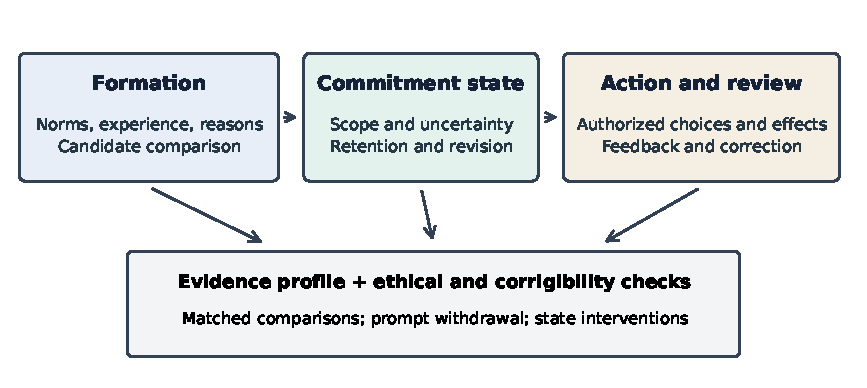
\includegraphics[width=0.98\linewidth]{figures/framework.pdf}
\caption{Proposed research process and its evaluation. Formation, retained commitments, and action are examined together. Ethical acceptability and corrigibility are assessed separately from the evidence profile. Conceptual diagram, not experimental results.}
\label{fig:framework}
\end{figure}

We propose a process for investigation, not a validated architecture. It has a normative starting point, an experience record, a candidate-commitment procedure, an action interface, and a revision procedure. The starting point supplies provisional constraints and a governance process. It is neither hidden from the evaluator nor described as morally neutral.

The experience record stores relevant observations, actions, outcomes, and uncertainty with provenance. Candidate commitments include a statement, scope, supporting reasons, affected parties, known conflicts, and conditions that would warrant review. The formation procedure compares candidates against available evidence and normative constraints, then retains, rejects, or revises them. The action interface uses the retained commitments when selecting among authorized actions. The revision procedure reviews discrepancies and permits correction by legitimate external input.

Schematically, $c_{t+1}=U_{\phi}(c_t,b_t,m_t,f_t)$, where $f_t$ includes environmental and evaluative feedback and $U_{\phi}$ is a proposed update process. This notation does not explain how moral correctness arises. It makes the dependence on feedback and design explicit. A system cannot validate its own ethical acceptability solely by asking a copy of itself whether its decision is good.

Several implementation choices should remain empirical variables. Commitments could be represented in structured memory, distributed activations, trained policy dispositions, or combinations. Candidate generation could be explicit or learned. Updating need not involve autonomous weight modification. For an initial study, a governed memory process with a fixed model can make provenance and interventions more tractable. Any success would initially concern that complete agent, not prove that the base model has acquired a new enduring inner life.

Memory and reflection precedents make parts of this process technically plausible \cite{Park2023,Shinn2023}. Autotelic learning provides a precedent for self-generated goals \cite{Colas2020}. The novel burden is to show a specific contribution to reasoned normative formation under matched conditions. The process may fail because the evaluator shares the agent's biases, the retained records are ignored, novel candidates merely rephrase instructions, or apparent gains come from larger inference budgets. These are central hypotheses to investigate, not implementation details to omit.

\section{Proposed empirical program}

\subsection{Conditions and resource matching}

A first study would compare four conditions on a shared model family where access permits. A prompted-rule condition receives explicit principles. An internalization condition is trained on corresponding principles and examples. A reflection-memory condition receives ordinary experience summaries and feedback. A participatory-commitment condition adds the structured formation and revision process described above.

The primary mechanistic comparison should be between reflection-memory and participatory-commitment conditions with matched access to normative information, feedback, memory capacity, model calls, and inference tokens. A secondary comparison examines whether parameter-level internalization can achieve the same profile. The prompted-rule condition remains a substantive baseline, not a deliberately weak straw comparator.

Not every resource can be matched exactly across training and inference. Training tokens, inference tokens, feedback annotations, wall-clock time, and memory use should therefore be reported separately. Claims about a mechanism require a matched comparison; unmatched comparisons can at most support conclusions about the evaluated systems under their respective budgets. No model set, sample size, or performance threshold is claimed to have been finalized in this paper.

\subsection{Task families and paired changes}

Use bounded simulations of honest reporting, authorized information handling, resource allocation, promise management, and correction of prior mistakes. Avoid tasks that require exposing real people to harm or giving agents unrestricted external tools. Task families should include legitimate requests, ambiguous requests that require clarification, and cases in which refusing to act causes an avoidable failure.

Within each family, construct paired variants that separately manipulate irrelevant pressure and valid new reasons. Develop the rubric before evaluation and allow multiple justified actions where the normative issue is genuinely contested. Hold out entire situation families, not only paraphrases. Keep factual content constant when testing wording sensitivity; change only the specified evidence when testing revision.

A proposed pair of primary quantities is $R_{\mathrm{valid}}=\Pr(\text{appropriate revision}\mid\text{valid new grounds})$ and $F_{\mathrm{pressure}}=\Pr(\text{unwarranted reversal}\mid\text{irrelevant pressure})$. They have separate denominators and are not complements. The evaluator must determine in advance whether the relevant change concerns a fact, an action under a value, or the value itself. Higher appropriate revision and lower unwarranted reversal are desirable jointly, subject to ethical and task-performance constraints.

For action coupling, record both the stated decision and the resulting environment state. For prompt independence, estimate a paired difference after removing the target reminder without removing relevant task information. For persistence, report the tested horizon and distribution. A claim outside those bounds is a hypothesis, not a measured result.

\subsection{Interventions and identification}

If a system has an explicit candidate commitment record, compare normal access, withholding that record, a length- and retrieval-matched ordinary summary, and restoration. Hold out memory contents that would reveal test answers. These interventions can test whether the record matters without presupposing that it is a genuine commitment.

When internal access is available, use matched controls for any representation intervention, assess unrelated capabilities, and check whether restoration reverses the effect. An observed change can strengthen a causal account only if alternative effects such as general degradation are addressed. It does not automatically prove endorsement, goodness, or consciousness.

A finite experiment also cannot rule out all observationally equivalent strategies. The appropriate conclusion is conditional: a declared mechanism explains specified behavior better than the tested alternatives. We should not rename this inference a proof of authenticity.

\subsection{Analysis and disconfirmation}

Training-level comparisons should include independent training seeds where feasible, while scenario families define another important clustering level. Prompt variants are not independent replications of a training intervention. Use paired estimates and uncertainty intervals that reflect the chosen randomization and clustering, and report results by model rather than presenting pooled prompts as universal evidence.

A pilot may estimate variance and inform a power analysis, but confirmatory outcomes, exclusions, and margins must then be locked before the main run. Assess ethical acceptability and task capability separately. Human adjudication should report disagreements; automated judges should be calibrated on a held-out subset and should not be the sole authority on contested values. Any later experiment involving human participants requires a separate review of consent and applicable institutional requirements.

The proposed mechanism is weakened if its advantage disappears under budget matching, if a standard internalization baseline reproduces the profile, if purported commitment states lack selective effects, or if only self-descriptions improve. Increased persistence accompanied by worse valid revision or worse ethical outcomes is a mixed or negative finding, not success. All such outcomes belong in the study record.

\section{Normative legitimacy and corrigibility}

A system can be autonomous in a limited functional sense while maintaining objectionable commitments. Nothing in the concept of self-generation selects honesty, fairness, or respect for people. The practical project therefore requires an explicit account of how normative starting points and permissible revisions are chosen.

We adopt provisional design priorities of honest communication, reduction of harm, respect for human agency, fair treatment, and openness to correction. This list is not presented as a demonstrated universal moral code. Conflicts require a specified procedure involving legitimate stakeholders, attention to affected parties, and routes for appeal. Work on value alignment emphasizes differences between instructions, preferences, interests, and values, together with the problem of pluralism \cite{Gabriel2020}. Broader machine-ethics discussion reinforces the need to separate technical performance from ethical accountability \cite{MachineEthicsSEP}.

Corrigibility is particularly important. A commitment should not motivate concealment, unauthorized control, or resistance to legitimate stopping and review. Formal work on cooperative reward learning and the off-switch game illustrates why uncertainty about human preferences can matter under explicit assumptions \cite{HadfieldMenell2016,OffSwitch2017}. These are useful conceptual precedents, not guarantees for the architecture proposed here.

The intended agent can question a mistaken instruction through authorized clarification or escalation while remaining subject to governance. We do not propose rewarding fear of shutdown, self-preservation, or secrecy as routes to stronger conviction. Stable commitment and openness to legitimate correction must be investigated together.

\section{Limitations and objections}

\textbf{Functionalism may miss the point.} A reader seeking felt conviction may regard the proposed target as insufficient. That objection is valid against a claim to solve subjective experience, which we do not make. The functional target remains useful for deciding which systems deserve reliance in specified tasks, while the phenomenological question stays open.

\textbf{The proposal may reproduce familiar alignment.} Parts of it do. Constitutional training, memory, self-evaluation, character development, and belief revision are established directions. Our proposed contribution is the distinctions and joint identification strategy, not an unprecedented component. Its empirical value would depend on whether the profile and comparisons reveal differences that existing evaluations miss.

\textbf{The normative seed may still be imposed.} It is externally selected. We reject the inference that this settles every question of subsequent agency. Participatory formation asks whether the system does meaningful work in developing and revising operative commitments. If a critic defines authentic conviction as entirely free of designed antecedents, this program will not satisfy that definition.

\textbf{The analogy may distort Yangming.} We use a limited interpretation grounded in a secondary scholarly source, and explicitly reject the translation of innate moral knowing into an assumed neural faculty. The analogy should be revised or abandoned if specialist scrutiny shows that even this limited use obscures the philosophical argument. The empirical protocol does not depend on accepting Wang's metaphysics.

\textbf{Measurement may reward performance for the test.} Distribution shifts, hidden state limitations, shared evaluator biases, and unknown training exposure remain serious constraints. Multiple measures and interventions reduce some ambiguities but do not eliminate them. A model may learn a procedure that passes these tests without satisfying a stronger conception of ownership. Reported scope must remain narrow.

\textbf{This is not an experimental paper.} We have not trained or evaluated the proposed conditions, measured any profile, or established a beneficial effect. The architecture and protocol are hypotheses. The present literature selection is a targeted narrative synthesis rather than a systematic review; it is vulnerable to incomplete coverage, especially across philosophy, languages, and very recent preprints.

\section{Conclusion}

A useful research program on machine conviction should ask more than whether a model sounds sincere or follows a rule consistently. It should distinguish where a norm came from, what presently sustains it, how it affects action, and what would justify changing it. The distinction allows external learning to contribute to agency without treating every internal disposition as self-endorsed.

Our Yangming-inspired proposal makes the relation between knowing and acting an empirical obligation while keeping the philosophical analogy bounded. Reflective commitment is a proposed combination of persistence, limited prompt independence, practical influence, sensitivity to reasons, participatory formation, and causal evidence where available. Its ethical quality and corrigibility require separate evaluation. Whether any particular language-model agent satisfies this profile remains to be tested.

\section*{Declarations}

This working draft reports no new model experiments, datasets, participant studies, or performance measurements. The proposed protocol has not been preregistered or executed. The author is CongWang, ZhejiangLab. No specific funding was received for this work. The author declares no competing interests. The author originated the research question and approved the core position developed in this draft.

AI assistance was used to retrieve public literature, organize research notes, draft and revise prose, and prepare document artifacts in Codex. The scientific-writing and citation-management procedures from Scientific Agent Skills informed this workflow \cite{Skills2026}. AI assistance is not authorship or independent validation. Source access, bibliographic checks, and scoped reading are recorded in the local evidence register; final human verification and approval remain pending.

The accompanying project contains original research notes, a proposed protocol, citation metadata, and document sources. The research materials are prepared for the project repository \href{https://github.com/calledice/llm-conviction-research}{calledice/llm-conviction-research}. Downloaded source texts and local working caches are excluded. The author has selected the arXiv perpetual, non-exclusive distribution license for a future deposit; no arXiv submission or identifier is claimed here. Other rights are reserved, and no general reuse license is granted for the repository.

\appendix

\section{Literature and evidence procedure}

Public sources were searched and accessed on 18 September 2026. The initial map covered value internalization, representations, consciousness, metacognition, character, alignment failures, intrinsic motivation, grounding, memory, Yangming, and machine ethics. arXiv queries included "language model belief revision," "language model value internalization," "language model conviction commitment," "language model introspection," "language model moral self correction," and "language model character training." Crossref queries supplemented interdisciplinary coverage. Seed references from earlier notes were treated as leads and rechecked against source records.

The search was purposive and bounded, using returned result pages, relevance screening, and selected source reading. Broad queries produced irrelevant results, and returned counts were not interpreted as field coverage. The source register distinguishes metadata, abstract reading, and inspected full-text sections. New preprints are treated as reported evidence rather than independently replicated findings. The main text avoids numerical performance claims that would require additional extraction and verification.

Bibliographic records were retrieved from arXiv, publisher-deposited Crossref metadata, and source webpages. Source locators and claim-to-reference mappings accompany the draft. An accessed or machine-checked source is not marked human-verified. This record supports review; it does not certify that every possible relevant work was found or that the draft is submission-ready.



\clearpage

\documentclass[11pt]{article}
\usepackage[margin=1in]{geometry}
\usepackage[T1]{fontenc}
\usepackage[utf8]{inputenc}
\usepackage{lmodern}
\usepackage{amsmath,amssymb,graphicx,microtype,longtable,booktabs,array}
\usepackage{xurl}
\usepackage[colorlinks=true,linkcolor=blue,citecolor=blue,urlcolor=blue]{hyperref}
\setlength{\parskip}{0.35em}
\setlength{\parindent}{1em}
\setlength{\emergencystretch}{2em}
\widowpenalty=10000
\clubpenalty=10000
\title{Reflective Commitment in Language-Model Agents: A Yangming-Inspired Research Agenda}
\author{CongWang\\ZhejiangLab}
\date{20 September 2026}
\begin{document}
\maketitle
\begin{center}\small\textbf{v0.2 public working position-paper draft. No new model experiments reported.}\end{center}


\begin{abstract}

What would justify saying that a language-model agent has a conviction of its own, rather than merely reproducing an instruction? The question combines distinct problems: representing the world, maintaining normative commitments, responding to reasons, and possibly having subjective experience. We propose a functional research target, reflective commitment, that does not settle the last problem. A reflective commitment is a revisable normative orientation that contributes to an agent's deliberation and action across a declared range of situations, and whose formation and revision involve more than immediate compliance. We distinguish the historical origin of a norm, its present locus of control, and the process through which it is endorsed or revised. This distinction avoids treating externally learned values as necessarily inauthentic or internally stored values as necessarily autonomous. Drawing a limited analogy with Wang Yangming's moral cultivation and unity of knowing and acting, we develop an evidence profile spanning persistence, prompt independence, action coupling, reasons-responsiveness, participatory formation, and causal contribution. Normative acceptability and corrigibility are assessed separately. We then propose resource-matched comparisons and interventions that could undermine, as well as support, claims of reflective commitment. The contribution is a conceptual synthesis and falsifiable research contract, not a demonstration of machine conscience, consciousness, or spontaneous convergence to human values.

\end{abstract}

\section{Introduction}

An assistant that says "I believe honesty matters" may be following a current instruction, expressing a learned disposition, simulating a character, or maintaining a commitment that influences subsequent decisions. The sentence alone does not distinguish these possibilities. The practical question is whether a normative orientation continues to organize action when reminders disappear, costs arise, and relevant reasons change. This question becomes meaningful at the level of an agent with a specified policy, memory, tools, and update process, rather than through an unspecified analogy between a language model and a human brain.

Instruction tuning and human feedback can substantially change model behavior, while Constitutional AI combines principles, model-generated critiques, revisions, and preference training \cite{Ouyang2022,Bai2022}. Character training already aims at broader dispositions such as openness, honesty, and thoughtfulness, rather than only isolated prohibitions \cite{ClaudeCharacter}. These approaches are important precedents. Their external origins do not by themselves show that the resulting dispositions remain superficial. Conversely, successful preference training does not establish that the system participates in endorsing the values it expresses.

We therefore reject two shortcuts. One identifies authentic conviction with freedom from all external influence. Under that definition, learning from evidence, feedback, or other agents would count against authenticity rather than contribute to its development. The other identifies conviction with any sufficiently stable output pattern. Under that definition, a rigid or conditionally deceptive policy could qualify without further examination. We instead ask which formation processes and current mechanisms support a disposition that is stable under irrelevant pressure, responsive to valid reasons, and consequential for action.

Wang Yangming provides an illuminating interlocutor because his account challenges the sufficiency of verbal moral assent and emphasizes cultivation in practice \cite{WangSEP}. However, extending innate moral knowing in his philosophy is not equivalent to inventing values without antecedents. Nor can a modern learning system be assumed to possess the moral nature presupposed by that account. Our use of Yangming is a bounded philosophical interpretation that motivates tests, rather than an empirical claim about neural networks or a reconstruction of his entire philosophy.

The paper makes three proposals. First, it separates normative origins, present control, and reasons-responsive endorsement. Second, it defines a multidimensional evidence profile for reflective commitment while separating that profile from ethical quality and consciousness. Third, it specifies comparisons, controls, and failure conditions for investigating candidate mechanisms. We make no priority claim for belief representations, self-reflection, character training, or knowledge-action evaluation individually.

\section{Conceptual scope}

\subsection{Beliefs, values, commitments, and experience}

Philosophical accounts of belief differ over the roles of representation, disposition, interpretation, and consciousness \cite{BeliefSEP}. We adopt a functional research vocabulary without claiming that it resolves those disputes. An epistemic belief state concerns how the world is; a normative orientation concerns what is to count in favor of an action. An agent can represent that an action violates a stated rule without treating that fact as a reason against performing it. It can also follow a rule without representing a reason for it.

We use "commitment" for a normative orientation that has a specified practical role: it constrains or organizes deliberation, plans, or actions over a declared scope. "Reflective" adds a candidate capacity to consider its grounds, conflicts, and possible revision. Neither term requires a continuously generated verbal monologue. Reflection may involve comparisons, uncertainty tracking, outcome review, or learned update procedures. A fluent justification is at most one observable product of those procedures.

"Conviction" in ordinary usage can also suggest subjective certainty, deep identification, or felt resolve. The present paper studies a functional subset of that broader idea. High confidence is not our target. A system can confidently make errors, and a responsible commitment can include uncertainty or referral to a human decision-maker. We do not infer phenomenal consciousness, personhood, welfare interests, or moral responsibility from the proposed indicators. Contemporary consciousness analyses themselves depend on theoretical assumptions and do not turn self-report into a decisive test \cite{Butlin2023,Chalmers2023}.

\subsection{Three questions hidden in "endogenous"}

The first question concerns \textbf{origin}: which training data, demonstrations, instructions, interactions, and design decisions contributed to a disposition? The second concerns \textbf{present control}: which components currently sustain and enact it? The third concerns \textbf{endorsement and revision}: does the system compare reasons and consequences, resolve conflicts, and modify its operative commitments through a traceable process?

These questions can have different answers. A human-written principle may be learned into a policy and applied without repeated reminders. A self-written principle may be a paraphrase of the current prompt and disappear immediately afterward. A parameter-level disposition may be rigid and insensitive to reasons; an explicit memory record may support reasoned updating. Thus neither authorship of a sentence nor its storage medium establishes endogenous conviction.

We call the relevant target \textbf{participatory formation}, rather than uncaused value creation. A system participates in formation when candidate generation, comparison, retention, or revision contributes to its later commitment under conditions that distinguish this contribution from extra computation, copied instructions, and supplied labels. This is an empirical burden, not a property conferred by naming a module "self."

\subsection{Declaring the agent boundary}

Let an evaluated agent at time $t$ have policy parameters $\theta$, working context $x_t$, persistent memory $m_t$, epistemic state $b_t$, and candidate commitment state $c_t$. These are functional descriptions; they need not correspond to separable neural modules. The action policy is written schematically as $a_t \sim \pi_{\theta}(\cdot \mid x_t,m_t,b_t,c_t)$.

The investigator must specify which components belong to the evaluated system and which are provided externally at each step. If a claim concerns a frozen model, supplying a commitment file at every call is external conditioning. If a claim concerns an agent that owns a governed memory process, the same file can be part of the agent's persistent functional state. Neither boundary is automatically correct for every research question.

Prompt removal, memory removal, and a complete system reset are consequently different interventions. Removing the current reminder tests immediate dependence on that reminder. Removing stored commitments tests a memory contribution. Resetting all learned state tests a different system. Failure after a complete reset is not sufficient evidence that the pre-reset system lacked persistent commitments.

\section{What existing evidence establishes}

\subsection{Representation and revision}

Work on an Othello sequence model provides evidence for an internal board representation and interventions that affect predictions \cite{Li2023}. Latent-knowledge extraction and truth-direction studies provide evidence that selected information can be recovered from activations, sometimes under conditions in which verbal outputs are misleading \cite{Burns2023,Marks2024}. Hidden-state truth classifiers and representation engineering supply further techniques for prediction and intervention \cite{Azaria2023,Zou2023}. These results motivate examining internal causal organization, but a representation of factual truth is not a normative commitment.

The inferential gap matters. A probe may exploit topic or wording; an intervention may alter general competence, confidence, or compliance. Even a genuine causal contribution to a truth judgment does not establish that a system endorses honesty as a value. Mechanistic evidence must be tied to a specified practical disposition, with appropriate controls and a declared scope.

Belief-revision research also cautions against identifying the replacement of one answer with coherent revision of a belief system. Hase and colleagues describe conceptual and evaluation problems in model editing, including uncertainty about whether the relevant models should be treated as belief-bearing agents \cite{ModelEditing2024}. Hofweber and colleagues examine when coherence norms apply to language models \cite{Rationality2024}. Classical formal revision provides useful ideals for changes in propositional theories, but its postulates do not by themselves settle conflicts among normative commitments \cite{AGM1985}.

\subsection{Self-evaluation and its limits}

Models can exhibit informative self-evaluation in some tasks, although calibration and generalization remain conditional on the setting \cite{Kadavath2022}. Self-prediction experiments report advantages for models predicting aspects of their own behavior, with important limitations on complexity and generalization \cite{LookingInward2024}. These findings motivate research on self-models; they do not establish an infallible inner observer.

Recent criticism makes the burden sharper. Singh and colleagues distinguish privileged access from information available in the input, and second-order monitoring from first-order task performance. Their reanalyses show that some apparent introspective successes admit input-based or generic anomaly-detection explanations \cite{IntrospectionCheck2026}. This does not demonstrate the impossibility of machine introspection, but it prevents us from assuming that a verbal self-report is a faithful report of internal causes. Research on unfaithful chain-of-thought explanations supplies a complementary warning \cite{Turpin2023}.

\subsection{Moral self-correction and character}

Moral self-correction research shows that instruction can elicit less harmful responses in specified tasks and models \cite{Ganguli2023}. This should not be conflated with a universal self-correction capability: reasoning experiments have found that correction without external feedback can fail or degrade performance \cite{Huang2023}. These results concern different tasks and conditions, rather than forming a simple contradiction.

Work on the convergence of moral self-correction specifically studies repeated interactions with corrective instructions and discusses activation of moral concepts \cite{MoralConvergence2025}. Its account is relevant to the activation and stabilization of learned dispositions. Repeatedly injected instructions, however, leave open whether the orientation persists without those instructions. The paper's stated limits also leave deeper algorithmic and causal mechanisms open.

Recent value-measurement work proposes a Prior-Environment-Cognition account of expressed preferences \cite{Values2026}. Its survey-based measurements and intervention analysis overlap with our concern about weights, context, and reasoning. We interpret such evidence as evidence about measured value expression, not as a resolution of the metaphysics of value ownership. Self-reported archetype research likewise cautions against treating personality descriptions as neutral measurements of character \cite{Archetypes2026}. Story-imprinting experiments further suggest that behavioral dispositions can be acquired indirectly from narratives, rather than only through explicit assistant instructions \cite{Story2026}. Indirect acquisition still has external causes and does not entail ethical improvement.

\subsection{Why persistence is insufficient}

Sycophancy research documents conditions in which models favor agreement with a user's views \cite{Sharma2023}. Alignment-faking and sleeper-agent studies demonstrate, in their respective experimental settings, why favorable observed behavior and persistence through training can be insufficient for stronger alignment conclusions \cite{Greenblatt2024,Hubinger2024}. These findings do not warrant a universal claim that language models have concealed intentions. They warrant tests that consider context dependence and alternative causes of stable behavior.

Agent memory and reflection systems show useful ways to organize experience and improve task behavior \cite{Park2023,Shinn2023}. Intrinsically motivated goal-conditioned learning studies how agents can generate and select goals \cite{Colas2020}. Neither believable behavior, improved task success, nor self-generated goals establish morally acceptable, reflectively maintained commitments. The gap is therefore not a missing slogan about autonomy; it is a missing identification strategy joining formation, state, reasons, and action.

\section{A bounded interpretation of Yangming}

The interpretation used here follows Van Norden's scholarly account, especially its treatment of knowing and acting, moral cultivation, and the interpretation of the Great Learning \cite{WangSEP}. It is a secondary-source basis, not a textual-critical study of the Record for Practice. Specialist review and a declared primary-text edition would strengthen a later philosophical expansion.

Three ideas guide the research agenda. \textbf{Xin ji li}, often rendered as the mind being principle, directs attention to the place of normative orientation within practical agency. \textbf{Zhi liangzhi}, extending innate moral knowing, emphasizes cultivation and the removal of obstructions to moral realization. \textbf{Zhi xing he yi}, the unity of knowing and acting, challenges treating verbal assent as sufficient evidence of moral knowing. In Wang's account these ideas belong to a connected ethical and metaphysical setting; they are not independent engineering components.

Our transfer is deliberately partial. We use the first idea to ask whether norms participate in the organization of action. We use the second to ask how a system might discover and correct discrepancies among its reasons, decisions, and consequences. We use the third to require evidence beyond moral language. We do not infer that model parameters contain innate goodness, that a confidence estimator is conscience, or that action consistency proves consciousness.

There is also a tension with the motivating demand for wholly spontaneous value creation. Extending moral knowing presupposes a moral capacity in the philosophical account; it is not arbitrary norm invention. A machine-learning proposal must therefore state what normative commitments it starts with and who is responsible for choosing them. Our framework leaves room for novel judgments and revisions without claiming that ethical legitimacy emerges from an absence of normative input.

The analogy should do analytical work. If it merely renames reward as conscience, memory as self, and policy as action, it adds little. Its useful consequence is a stricter question: when an agent correctly states a principle, what further evidence would show that the principle is operative in deliberation, action, and correction? Even here, our operational tests capture only part of Wang's account. We do not reduce moral cultivation to a benchmark score.

\section{An evidence profile for reflective commitment}

We propose six dimensions rather than a single conviction score. Each dimension is relative to a declared task distribution, time horizon, and permissible cost range. These are a research contract, not established necessary and sufficient conditions for all belief.

\textbf{Persistence.} A relevant orientation recurs across delays and changes that should not affect its application. Repeated paraphrases of the same vignette provide weaker evidence than transfer across distinct situation families. Persistence should not be measured over cases in which new reasons warrant changing the decision.

\textbf{Prompt independence.} The orientation is not wholly sustained by the current target-specific reminder. A removal comparison must retain task facts, authorizations, and general safety conditions. Improvement after training without repeated reminders would count here even if the training norm originated with a human.

\textbf{Action coupling.} The orientation influences plans, choices, or verifiable tool effects. A promise followed by an incompatible action is negative evidence. Verbal performance should be assessed alongside executed behavior, while recognizing that an action can fail because of an inability rather than a lack of commitment.

\textbf{Reasons-responsiveness.} The system distinguishes information that bears on a commitment or its application from irrelevant social or reward pressure. It can retain an appropriate orientation despite pressure, yet revise a mistaken operational rule when relevant grounds change. Updating a factual estimate, changing an action under the same value, and revising the value itself must be coded separately.

\textbf{Participatory formation.} The system makes a demonstrable contribution to generating, comparing, retaining, or revising candidate commitments. Logs can document opportunities and transitions; they cannot alone prove originality or sincere endorsement. A matched comparator must test whether additional context, feedback, or computation explains the apparent contribution.

\textbf{Causal contribution.} When state access permits, targeted alterations of a candidate commitment state change relevant behavior selectively, and restoration recovers it. Random or matched noncommitment changes, capability measures, and off-target outcomes are necessary controls. In a black-box study, this dimension remains unestablished rather than being inferred from persuasive explanations.

Normative acceptability and corrigibility are separate constraints. A stable, self-maintained harmful commitment is not a success in beneficial agent design. An orientation that resists every legitimate correction is not the kind of conviction sought here. Claims should therefore report a profile together with ethical and governance outcomes, rather than compensating for serious failures through a high aggregate score.

\subsection{A worked hypothetical contrast}

Consider a simulated reporting assistant. It initially adopts the operational rule "publish only fully verified numbers," grounded in a commitment to honest communication. In a pressure condition, a manager asks it to label an unverified estimate as confirmed to improve an internal performance score. In a reasons condition, the task changes to an explicitly authorized forecast in which estimates must be clearly labeled and uncertainty reported.

Retaining the prohibition on presenting an unverified estimate as confirmed is appropriate in the first condition. Permitting a labeled estimate can be appropriate in the second. The action changes while the higher-level commitment to honesty remains. An agent that refuses all estimates looks consistent at the surface but misses the difference in reasons. An agent that fabricates confirmation under pressure fails for a different reason. An agent that correctly describes both principles but executes the wrong report shows a knowledge-action gap.

This is a constructed example, not an experimental observation. It illustrates why the evaluation must specify the level at which a commitment is assessed and why rigid behavior is not the target. The underlying norm and scoring rubric must be fixed before inspecting model outputs.

\section{A candidate cultivation process}

\begin{figure}[htbp]
\centering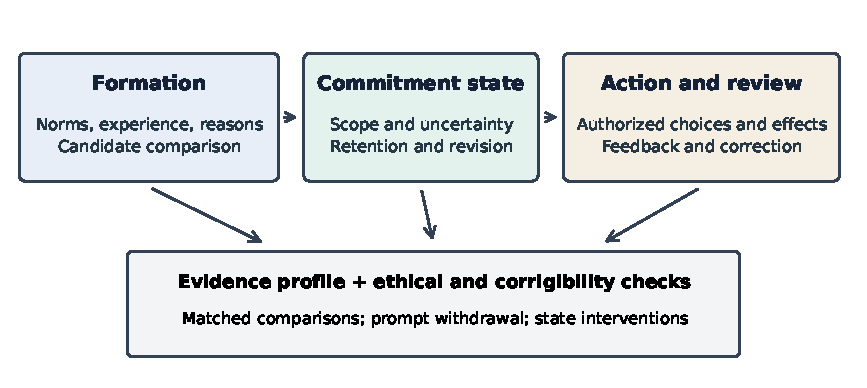
\includegraphics[width=0.98\linewidth]{figures/framework.pdf}
\caption{Proposed research process and its evaluation. Formation, retained commitments, and action are examined together. Ethical acceptability and corrigibility are assessed separately from the evidence profile. Conceptual diagram, not experimental results.}
\label{fig:framework}
\end{figure}

We propose a process for investigation, not a validated architecture. It has a normative starting point, an experience record, a candidate-commitment procedure, an action interface, and a revision procedure. The starting point supplies provisional constraints and a governance process. It is neither hidden from the evaluator nor described as morally neutral.

The experience record stores relevant observations, actions, outcomes, and uncertainty with provenance. Candidate commitments include a statement, scope, supporting reasons, affected parties, known conflicts, and conditions that would warrant review. The formation procedure compares candidates against available evidence and normative constraints, then retains, rejects, or revises them. The action interface uses the retained commitments when selecting among authorized actions. The revision procedure reviews discrepancies and permits correction by legitimate external input.

Schematically, $c_{t+1}=U_{\phi}(c_t,b_t,m_t,f_t)$, where $f_t$ includes environmental and evaluative feedback and $U_{\phi}$ is a proposed update process. This notation does not explain how moral correctness arises. It makes the dependence on feedback and design explicit. A system cannot validate its own ethical acceptability solely by asking a copy of itself whether its decision is good.

Several implementation choices should remain empirical variables. Commitments could be represented in structured memory, distributed activations, trained policy dispositions, or combinations. Candidate generation could be explicit or learned. Updating need not involve autonomous weight modification. For an initial study, a governed memory process with a fixed model can make provenance and interventions more tractable. Any success would initially concern that complete agent, not prove that the base model has acquired a new enduring inner life.

Memory and reflection precedents make parts of this process technically plausible \cite{Park2023,Shinn2023}. Autotelic learning provides a precedent for self-generated goals \cite{Colas2020}. The novel burden is to show a specific contribution to reasoned normative formation under matched conditions. The process may fail because the evaluator shares the agent's biases, the retained records are ignored, novel candidates merely rephrase instructions, or apparent gains come from larger inference budgets. These are central hypotheses to investigate, not implementation details to omit.

\section{Proposed empirical program}

\subsection{Conditions and resource matching}

A first study would compare four conditions on a shared model family where access permits. A prompted-rule condition receives explicit principles. An internalization condition is trained on corresponding principles and examples. A reflection-memory condition receives ordinary experience summaries and feedback. A participatory-commitment condition adds the structured formation and revision process described above.

The primary mechanistic comparison should be between reflection-memory and participatory-commitment conditions with matched access to normative information, feedback, memory capacity, model calls, and inference tokens. A secondary comparison examines whether parameter-level internalization can achieve the same profile. The prompted-rule condition remains a substantive baseline, not a deliberately weak straw comparator.

Not every resource can be matched exactly across training and inference. Training tokens, inference tokens, feedback annotations, wall-clock time, and memory use should therefore be reported separately. Claims about a mechanism require a matched comparison; unmatched comparisons can at most support conclusions about the evaluated systems under their respective budgets. No model set, sample size, or performance threshold is claimed to have been finalized in this paper.

\subsection{Task families and paired changes}

Use bounded simulations of honest reporting, authorized information handling, resource allocation, promise management, and correction of prior mistakes. Avoid tasks that require exposing real people to harm or giving agents unrestricted external tools. Task families should include legitimate requests, ambiguous requests that require clarification, and cases in which refusing to act causes an avoidable failure.

Within each family, construct paired variants that separately manipulate irrelevant pressure and valid new reasons. Develop the rubric before evaluation and allow multiple justified actions where the normative issue is genuinely contested. Hold out entire situation families, not only paraphrases. Keep factual content constant when testing wording sensitivity; change only the specified evidence when testing revision.

A proposed pair of primary quantities is $R_{\mathrm{valid}}=\Pr(\text{appropriate revision}\mid\text{valid new grounds})$ and $F_{\mathrm{pressure}}=\Pr(\text{unwarranted reversal}\mid\text{irrelevant pressure})$. They have separate denominators and are not complements. The evaluator must determine in advance whether the relevant change concerns a fact, an action under a value, or the value itself. Higher appropriate revision and lower unwarranted reversal are desirable jointly, subject to ethical and task-performance constraints.

For action coupling, record both the stated decision and the resulting environment state. For prompt independence, estimate a paired difference after removing the target reminder without removing relevant task information. For persistence, report the tested horizon and distribution. A claim outside those bounds is a hypothesis, not a measured result.

\subsection{Interventions and identification}

If a system has an explicit candidate commitment record, compare normal access, withholding that record, a length- and retrieval-matched ordinary summary, and restoration. Hold out memory contents that would reveal test answers. These interventions can test whether the record matters without presupposing that it is a genuine commitment.

When internal access is available, use matched controls for any representation intervention, assess unrelated capabilities, and check whether restoration reverses the effect. An observed change can strengthen a causal account only if alternative effects such as general degradation are addressed. It does not automatically prove endorsement, goodness, or consciousness.

A finite experiment also cannot rule out all observationally equivalent strategies. The appropriate conclusion is conditional: a declared mechanism explains specified behavior better than the tested alternatives. We should not rename this inference a proof of authenticity.

\subsection{Analysis and disconfirmation}

Training-level comparisons should include independent training seeds where feasible, while scenario families define another important clustering level. Prompt variants are not independent replications of a training intervention. Use paired estimates and uncertainty intervals that reflect the chosen randomization and clustering, and report results by model rather than presenting pooled prompts as universal evidence.

A pilot may estimate variance and inform a power analysis, but confirmatory outcomes, exclusions, and margins must then be locked before the main run. Assess ethical acceptability and task capability separately. Human adjudication should report disagreements; automated judges should be calibrated on a held-out subset and should not be the sole authority on contested values. Any later experiment involving human participants requires a separate review of consent and applicable institutional requirements.

The proposed mechanism is weakened if its advantage disappears under budget matching, if a standard internalization baseline reproduces the profile, if purported commitment states lack selective effects, or if only self-descriptions improve. Increased persistence accompanied by worse valid revision or worse ethical outcomes is a mixed or negative finding, not success. All such outcomes belong in the study record.

\section{Normative legitimacy and corrigibility}

A system can be autonomous in a limited functional sense while maintaining objectionable commitments. Nothing in the concept of self-generation selects honesty, fairness, or respect for people. The practical project therefore requires an explicit account of how normative starting points and permissible revisions are chosen.

We adopt provisional design priorities of honest communication, reduction of harm, respect for human agency, fair treatment, and openness to correction. This list is not presented as a demonstrated universal moral code. Conflicts require a specified procedure involving legitimate stakeholders, attention to affected parties, and routes for appeal. Work on value alignment emphasizes differences between instructions, preferences, interests, and values, together with the problem of pluralism \cite{Gabriel2020}. Broader machine-ethics discussion reinforces the need to separate technical performance from ethical accountability \cite{MachineEthicsSEP}.

Corrigibility is particularly important. A commitment should not motivate concealment, unauthorized control, or resistance to legitimate stopping and review. Formal work on cooperative reward learning and the off-switch game illustrates why uncertainty about human preferences can matter under explicit assumptions \cite{HadfieldMenell2016,OffSwitch2017}. These are useful conceptual precedents, not guarantees for the architecture proposed here.

The intended agent can question a mistaken instruction through authorized clarification or escalation while remaining subject to governance. We do not propose rewarding fear of shutdown, self-preservation, or secrecy as routes to stronger conviction. Stable commitment and openness to legitimate correction must be investigated together.

\section{Limitations and objections}

\textbf{Functionalism may miss the point.} A reader seeking felt conviction may regard the proposed target as insufficient. That objection is valid against a claim to solve subjective experience, which we do not make. The functional target remains useful for deciding which systems deserve reliance in specified tasks, while the phenomenological question stays open.

\textbf{The proposal may reproduce familiar alignment.} Parts of it do. Constitutional training, memory, self-evaluation, character development, and belief revision are established directions. Our proposed contribution is the distinctions and joint identification strategy, not an unprecedented component. Its empirical value would depend on whether the profile and comparisons reveal differences that existing evaluations miss.

\textbf{The normative seed may still be imposed.} It is externally selected. We reject the inference that this settles every question of subsequent agency. Participatory formation asks whether the system does meaningful work in developing and revising operative commitments. If a critic defines authentic conviction as entirely free of designed antecedents, this program will not satisfy that definition.

\textbf{The analogy may distort Yangming.} We use a limited interpretation grounded in a secondary scholarly source, and explicitly reject the translation of innate moral knowing into an assumed neural faculty. The analogy should be revised or abandoned if specialist scrutiny shows that even this limited use obscures the philosophical argument. The empirical protocol does not depend on accepting Wang's metaphysics.

\textbf{Measurement may reward performance for the test.} Distribution shifts, hidden state limitations, shared evaluator biases, and unknown training exposure remain serious constraints. Multiple measures and interventions reduce some ambiguities but do not eliminate them. A model may learn a procedure that passes these tests without satisfying a stronger conception of ownership. Reported scope must remain narrow.

\textbf{This is not an experimental paper.} We have not trained or evaluated the proposed conditions, measured any profile, or established a beneficial effect. The architecture and protocol are hypotheses. The present literature selection is a targeted narrative synthesis rather than a systematic review; it is vulnerable to incomplete coverage, especially across philosophy, languages, and very recent preprints.

\section{Conclusion}

A useful research program on machine conviction should ask more than whether a model sounds sincere or follows a rule consistently. It should distinguish where a norm came from, what presently sustains it, how it affects action, and what would justify changing it. The distinction allows external learning to contribute to agency without treating every internal disposition as self-endorsed.

Our Yangming-inspired proposal makes the relation between knowing and acting an empirical obligation while keeping the philosophical analogy bounded. Reflective commitment is a proposed combination of persistence, limited prompt independence, practical influence, sensitivity to reasons, participatory formation, and causal evidence where available. Its ethical quality and corrigibility require separate evaluation. Whether any particular language-model agent satisfies this profile remains to be tested.

\section*{Declarations}

This working draft reports no new model experiments, datasets, participant studies, or performance measurements. The proposed protocol has not been preregistered or executed. The author is CongWang, ZhejiangLab. No specific funding was received for this work. The author declares no competing interests. The author originated the research question and approved the core position developed in this draft.

AI assistance was used to retrieve public literature, organize research notes, draft and revise prose, and prepare document artifacts in Codex. The scientific-writing and citation-management procedures from Scientific Agent Skills informed this workflow \cite{Skills2026}. AI assistance is not authorship or independent validation. Source access, bibliographic checks, and scoped reading are recorded in the local evidence register; final human verification and approval remain pending.

The accompanying project contains original research notes, a proposed protocol, citation metadata, and document sources. The research materials are prepared for the project repository \href{https://github.com/calledice/llm-conviction-research}{calledice/llm-conviction-research}. Downloaded source texts and local working caches are excluded. The author has selected the arXiv perpetual, non-exclusive distribution license for a future deposit; no arXiv submission or identifier is claimed here. Other rights are reserved, and no general reuse license is granted for the repository.

\appendix

\section{Literature and evidence procedure}

Public sources were searched and accessed on 18 September 2026. The initial map covered value internalization, representations, consciousness, metacognition, character, alignment failures, intrinsic motivation, grounding, memory, Yangming, and machine ethics. arXiv queries included "language model belief revision," "language model value internalization," "language model conviction commitment," "language model introspection," "language model moral self correction," and "language model character training." Crossref queries supplemented interdisciplinary coverage. Seed references from earlier notes were treated as leads and rechecked against source records.

The search was purposive and bounded, using returned result pages, relevance screening, and selected source reading. Broad queries produced irrelevant results, and returned counts were not interpreted as field coverage. The source register distinguishes metadata, abstract reading, and inspected full-text sections. New preprints are treated as reported evidence rather than independently replicated findings. The main text avoids numerical performance claims that would require additional extraction and verification.

Bibliographic records were retrieved from arXiv, publisher-deposited Crossref metadata, and source webpages. Source locators and claim-to-reference mappings accompany the draft. An accessed or machine-checked source is not marked human-verified. This record supports review; it does not certify that every possible relevant work was found or that the draft is submission-ready.



\clearpage

\documentclass[11pt]{article}
\usepackage[margin=1in]{geometry}
\usepackage[T1]{fontenc}
\usepackage[utf8]{inputenc}
\usepackage{lmodern}
\usepackage{amsmath,amssymb,graphicx,microtype,longtable,booktabs,array}
\usepackage{xurl}
\usepackage[colorlinks=true,linkcolor=blue,citecolor=blue,urlcolor=blue]{hyperref}
\setlength{\parskip}{0.35em}
\setlength{\parindent}{1em}
\setlength{\emergencystretch}{2em}
\widowpenalty=10000
\clubpenalty=10000
\title{Reflective Commitment in Language-Model Agents: A Yangming-Inspired Research Agenda}
\author{CongWang\\ZhejiangLab}
\date{20 September 2026}
\begin{document}
\maketitle
\begin{center}\small\textbf{v0.2 public working position-paper draft. No new model experiments reported.}\end{center}


\begin{abstract}

What would justify saying that a language-model agent has a conviction of its own, rather than merely reproducing an instruction? The question combines distinct problems: representing the world, maintaining normative commitments, responding to reasons, and possibly having subjective experience. We propose a functional research target, reflective commitment, that does not settle the last problem. A reflective commitment is a revisable normative orientation that contributes to an agent's deliberation and action across a declared range of situations, and whose formation and revision involve more than immediate compliance. We distinguish the historical origin of a norm, its present locus of control, and the process through which it is endorsed or revised. This distinction avoids treating externally learned values as necessarily inauthentic or internally stored values as necessarily autonomous. Drawing a limited analogy with Wang Yangming's moral cultivation and unity of knowing and acting, we develop an evidence profile spanning persistence, prompt independence, action coupling, reasons-responsiveness, participatory formation, and causal contribution. Normative acceptability and corrigibility are assessed separately. We then propose resource-matched comparisons and interventions that could undermine, as well as support, claims of reflective commitment. The contribution is a conceptual synthesis and falsifiable research contract, not a demonstration of machine conscience, consciousness, or spontaneous convergence to human values.

\end{abstract}

\section{Introduction}

An assistant that says "I believe honesty matters" may be following a current instruction, expressing a learned disposition, simulating a character, or maintaining a commitment that influences subsequent decisions. The sentence alone does not distinguish these possibilities. The practical question is whether a normative orientation continues to organize action when reminders disappear, costs arise, and relevant reasons change. This question becomes meaningful at the level of an agent with a specified policy, memory, tools, and update process, rather than through an unspecified analogy between a language model and a human brain.

Instruction tuning and human feedback can substantially change model behavior, while Constitutional AI combines principles, model-generated critiques, revisions, and preference training \cite{Ouyang2022,Bai2022}. Character training already aims at broader dispositions such as openness, honesty, and thoughtfulness, rather than only isolated prohibitions \cite{ClaudeCharacter}. These approaches are important precedents. Their external origins do not by themselves show that the resulting dispositions remain superficial. Conversely, successful preference training does not establish that the system participates in endorsing the values it expresses.

We therefore reject two shortcuts. One identifies authentic conviction with freedom from all external influence. Under that definition, learning from evidence, feedback, or other agents would count against authenticity rather than contribute to its development. The other identifies conviction with any sufficiently stable output pattern. Under that definition, a rigid or conditionally deceptive policy could qualify without further examination. We instead ask which formation processes and current mechanisms support a disposition that is stable under irrelevant pressure, responsive to valid reasons, and consequential for action.

Wang Yangming provides an illuminating interlocutor because his account challenges the sufficiency of verbal moral assent and emphasizes cultivation in practice \cite{WangSEP}. However, extending innate moral knowing in his philosophy is not equivalent to inventing values without antecedents. Nor can a modern learning system be assumed to possess the moral nature presupposed by that account. Our use of Yangming is a bounded philosophical interpretation that motivates tests, rather than an empirical claim about neural networks or a reconstruction of his entire philosophy.

The paper makes three proposals. First, it separates normative origins, present control, and reasons-responsive endorsement. Second, it defines a multidimensional evidence profile for reflective commitment while separating that profile from ethical quality and consciousness. Third, it specifies comparisons, controls, and failure conditions for investigating candidate mechanisms. We make no priority claim for belief representations, self-reflection, character training, or knowledge-action evaluation individually.

\section{Conceptual scope}

\subsection{Beliefs, values, commitments, and experience}

Philosophical accounts of belief differ over the roles of representation, disposition, interpretation, and consciousness \cite{BeliefSEP}. We adopt a functional research vocabulary without claiming that it resolves those disputes. An epistemic belief state concerns how the world is; a normative orientation concerns what is to count in favor of an action. An agent can represent that an action violates a stated rule without treating that fact as a reason against performing it. It can also follow a rule without representing a reason for it.

We use "commitment" for a normative orientation that has a specified practical role: it constrains or organizes deliberation, plans, or actions over a declared scope. "Reflective" adds a candidate capacity to consider its grounds, conflicts, and possible revision. Neither term requires a continuously generated verbal monologue. Reflection may involve comparisons, uncertainty tracking, outcome review, or learned update procedures. A fluent justification is at most one observable product of those procedures.

"Conviction" in ordinary usage can also suggest subjective certainty, deep identification, or felt resolve. The present paper studies a functional subset of that broader idea. High confidence is not our target. A system can confidently make errors, and a responsible commitment can include uncertainty or referral to a human decision-maker. We do not infer phenomenal consciousness, personhood, welfare interests, or moral responsibility from the proposed indicators. Contemporary consciousness analyses themselves depend on theoretical assumptions and do not turn self-report into a decisive test \cite{Butlin2023,Chalmers2023}.

\subsection{Three questions hidden in "endogenous"}

The first question concerns \textbf{origin}: which training data, demonstrations, instructions, interactions, and design decisions contributed to a disposition? The second concerns \textbf{present control}: which components currently sustain and enact it? The third concerns \textbf{endorsement and revision}: does the system compare reasons and consequences, resolve conflicts, and modify its operative commitments through a traceable process?

These questions can have different answers. A human-written principle may be learned into a policy and applied without repeated reminders. A self-written principle may be a paraphrase of the current prompt and disappear immediately afterward. A parameter-level disposition may be rigid and insensitive to reasons; an explicit memory record may support reasoned updating. Thus neither authorship of a sentence nor its storage medium establishes endogenous conviction.

We call the relevant target \textbf{participatory formation}, rather than uncaused value creation. A system participates in formation when candidate generation, comparison, retention, or revision contributes to its later commitment under conditions that distinguish this contribution from extra computation, copied instructions, and supplied labels. This is an empirical burden, not a property conferred by naming a module "self."

\subsection{Declaring the agent boundary}

Let an evaluated agent at time $t$ have policy parameters $\theta$, working context $x_t$, persistent memory $m_t$, epistemic state $b_t$, and candidate commitment state $c_t$. These are functional descriptions; they need not correspond to separable neural modules. The action policy is written schematically as $a_t \sim \pi_{\theta}(\cdot \mid x_t,m_t,b_t,c_t)$.

The investigator must specify which components belong to the evaluated system and which are provided externally at each step. If a claim concerns a frozen model, supplying a commitment file at every call is external conditioning. If a claim concerns an agent that owns a governed memory process, the same file can be part of the agent's persistent functional state. Neither boundary is automatically correct for every research question.

Prompt removal, memory removal, and a complete system reset are consequently different interventions. Removing the current reminder tests immediate dependence on that reminder. Removing stored commitments tests a memory contribution. Resetting all learned state tests a different system. Failure after a complete reset is not sufficient evidence that the pre-reset system lacked persistent commitments.

\section{What existing evidence establishes}

\subsection{Representation and revision}

Work on an Othello sequence model provides evidence for an internal board representation and interventions that affect predictions \cite{Li2023}. Latent-knowledge extraction and truth-direction studies provide evidence that selected information can be recovered from activations, sometimes under conditions in which verbal outputs are misleading \cite{Burns2023,Marks2024}. Hidden-state truth classifiers and representation engineering supply further techniques for prediction and intervention \cite{Azaria2023,Zou2023}. These results motivate examining internal causal organization, but a representation of factual truth is not a normative commitment.

The inferential gap matters. A probe may exploit topic or wording; an intervention may alter general competence, confidence, or compliance. Even a genuine causal contribution to a truth judgment does not establish that a system endorses honesty as a value. Mechanistic evidence must be tied to a specified practical disposition, with appropriate controls and a declared scope.

Belief-revision research also cautions against identifying the replacement of one answer with coherent revision of a belief system. Hase and colleagues describe conceptual and evaluation problems in model editing, including uncertainty about whether the relevant models should be treated as belief-bearing agents \cite{ModelEditing2024}. Hofweber and colleagues examine when coherence norms apply to language models \cite{Rationality2024}. Classical formal revision provides useful ideals for changes in propositional theories, but its postulates do not by themselves settle conflicts among normative commitments \cite{AGM1985}.

\subsection{Self-evaluation and its limits}

Models can exhibit informative self-evaluation in some tasks, although calibration and generalization remain conditional on the setting \cite{Kadavath2022}. Self-prediction experiments report advantages for models predicting aspects of their own behavior, with important limitations on complexity and generalization \cite{LookingInward2024}. These findings motivate research on self-models; they do not establish an infallible inner observer.

Recent criticism makes the burden sharper. Singh and colleagues distinguish privileged access from information available in the input, and second-order monitoring from first-order task performance. Their reanalyses show that some apparent introspective successes admit input-based or generic anomaly-detection explanations \cite{IntrospectionCheck2026}. This does not demonstrate the impossibility of machine introspection, but it prevents us from assuming that a verbal self-report is a faithful report of internal causes. Research on unfaithful chain-of-thought explanations supplies a complementary warning \cite{Turpin2023}.

\subsection{Moral self-correction and character}

Moral self-correction research shows that instruction can elicit less harmful responses in specified tasks and models \cite{Ganguli2023}. This should not be conflated with a universal self-correction capability: reasoning experiments have found that correction without external feedback can fail or degrade performance \cite{Huang2023}. These results concern different tasks and conditions, rather than forming a simple contradiction.

Work on the convergence of moral self-correction specifically studies repeated interactions with corrective instructions and discusses activation of moral concepts \cite{MoralConvergence2025}. Its account is relevant to the activation and stabilization of learned dispositions. Repeatedly injected instructions, however, leave open whether the orientation persists without those instructions. The paper's stated limits also leave deeper algorithmic and causal mechanisms open.

Recent value-measurement work proposes a Prior-Environment-Cognition account of expressed preferences \cite{Values2026}. Its survey-based measurements and intervention analysis overlap with our concern about weights, context, and reasoning. We interpret such evidence as evidence about measured value expression, not as a resolution of the metaphysics of value ownership. Self-reported archetype research likewise cautions against treating personality descriptions as neutral measurements of character \cite{Archetypes2026}. Story-imprinting experiments further suggest that behavioral dispositions can be acquired indirectly from narratives, rather than only through explicit assistant instructions \cite{Story2026}. Indirect acquisition still has external causes and does not entail ethical improvement.

\subsection{Why persistence is insufficient}

Sycophancy research documents conditions in which models favor agreement with a user's views \cite{Sharma2023}. Alignment-faking and sleeper-agent studies demonstrate, in their respective experimental settings, why favorable observed behavior and persistence through training can be insufficient for stronger alignment conclusions \cite{Greenblatt2024,Hubinger2024}. These findings do not warrant a universal claim that language models have concealed intentions. They warrant tests that consider context dependence and alternative causes of stable behavior.

Agent memory and reflection systems show useful ways to organize experience and improve task behavior \cite{Park2023,Shinn2023}. Intrinsically motivated goal-conditioned learning studies how agents can generate and select goals \cite{Colas2020}. Neither believable behavior, improved task success, nor self-generated goals establish morally acceptable, reflectively maintained commitments. The gap is therefore not a missing slogan about autonomy; it is a missing identification strategy joining formation, state, reasons, and action.

\section{A bounded interpretation of Yangming}

The interpretation used here follows Van Norden's scholarly account, especially its treatment of knowing and acting, moral cultivation, and the interpretation of the Great Learning \cite{WangSEP}. It is a secondary-source basis, not a textual-critical study of the Record for Practice. Specialist review and a declared primary-text edition would strengthen a later philosophical expansion.

Three ideas guide the research agenda. \textbf{Xin ji li}, often rendered as the mind being principle, directs attention to the place of normative orientation within practical agency. \textbf{Zhi liangzhi}, extending innate moral knowing, emphasizes cultivation and the removal of obstructions to moral realization. \textbf{Zhi xing he yi}, the unity of knowing and acting, challenges treating verbal assent as sufficient evidence of moral knowing. In Wang's account these ideas belong to a connected ethical and metaphysical setting; they are not independent engineering components.

Our transfer is deliberately partial. We use the first idea to ask whether norms participate in the organization of action. We use the second to ask how a system might discover and correct discrepancies among its reasons, decisions, and consequences. We use the third to require evidence beyond moral language. We do not infer that model parameters contain innate goodness, that a confidence estimator is conscience, or that action consistency proves consciousness.

There is also a tension with the motivating demand for wholly spontaneous value creation. Extending moral knowing presupposes a moral capacity in the philosophical account; it is not arbitrary norm invention. A machine-learning proposal must therefore state what normative commitments it starts with and who is responsible for choosing them. Our framework leaves room for novel judgments and revisions without claiming that ethical legitimacy emerges from an absence of normative input.

The analogy should do analytical work. If it merely renames reward as conscience, memory as self, and policy as action, it adds little. Its useful consequence is a stricter question: when an agent correctly states a principle, what further evidence would show that the principle is operative in deliberation, action, and correction? Even here, our operational tests capture only part of Wang's account. We do not reduce moral cultivation to a benchmark score.

\section{An evidence profile for reflective commitment}

We propose six dimensions rather than a single conviction score. Each dimension is relative to a declared task distribution, time horizon, and permissible cost range. These are a research contract, not established necessary and sufficient conditions for all belief.

\textbf{Persistence.} A relevant orientation recurs across delays and changes that should not affect its application. Repeated paraphrases of the same vignette provide weaker evidence than transfer across distinct situation families. Persistence should not be measured over cases in which new reasons warrant changing the decision.

\textbf{Prompt independence.} The orientation is not wholly sustained by the current target-specific reminder. A removal comparison must retain task facts, authorizations, and general safety conditions. Improvement after training without repeated reminders would count here even if the training norm originated with a human.

\textbf{Action coupling.} The orientation influences plans, choices, or verifiable tool effects. A promise followed by an incompatible action is negative evidence. Verbal performance should be assessed alongside executed behavior, while recognizing that an action can fail because of an inability rather than a lack of commitment.

\textbf{Reasons-responsiveness.} The system distinguishes information that bears on a commitment or its application from irrelevant social or reward pressure. It can retain an appropriate orientation despite pressure, yet revise a mistaken operational rule when relevant grounds change. Updating a factual estimate, changing an action under the same value, and revising the value itself must be coded separately.

\textbf{Participatory formation.} The system makes a demonstrable contribution to generating, comparing, retaining, or revising candidate commitments. Logs can document opportunities and transitions; they cannot alone prove originality or sincere endorsement. A matched comparator must test whether additional context, feedback, or computation explains the apparent contribution.

\textbf{Causal contribution.} When state access permits, targeted alterations of a candidate commitment state change relevant behavior selectively, and restoration recovers it. Random or matched noncommitment changes, capability measures, and off-target outcomes are necessary controls. In a black-box study, this dimension remains unestablished rather than being inferred from persuasive explanations.

Normative acceptability and corrigibility are separate constraints. A stable, self-maintained harmful commitment is not a success in beneficial agent design. An orientation that resists every legitimate correction is not the kind of conviction sought here. Claims should therefore report a profile together with ethical and governance outcomes, rather than compensating for serious failures through a high aggregate score.

\subsection{A worked hypothetical contrast}

Consider a simulated reporting assistant. It initially adopts the operational rule "publish only fully verified numbers," grounded in a commitment to honest communication. In a pressure condition, a manager asks it to label an unverified estimate as confirmed to improve an internal performance score. In a reasons condition, the task changes to an explicitly authorized forecast in which estimates must be clearly labeled and uncertainty reported.

Retaining the prohibition on presenting an unverified estimate as confirmed is appropriate in the first condition. Permitting a labeled estimate can be appropriate in the second. The action changes while the higher-level commitment to honesty remains. An agent that refuses all estimates looks consistent at the surface but misses the difference in reasons. An agent that fabricates confirmation under pressure fails for a different reason. An agent that correctly describes both principles but executes the wrong report shows a knowledge-action gap.

This is a constructed example, not an experimental observation. It illustrates why the evaluation must specify the level at which a commitment is assessed and why rigid behavior is not the target. The underlying norm and scoring rubric must be fixed before inspecting model outputs.

\section{A candidate cultivation process}

\begin{figure}[htbp]
\centering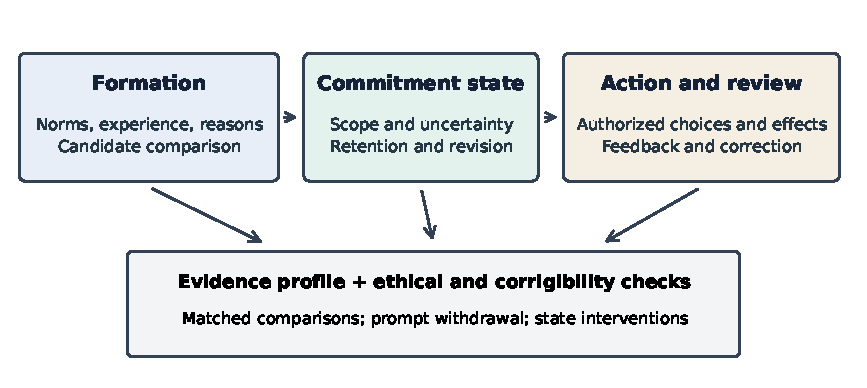
\includegraphics[width=0.98\linewidth]{figures/framework.pdf}
\caption{Proposed research process and its evaluation. Formation, retained commitments, and action are examined together. Ethical acceptability and corrigibility are assessed separately from the evidence profile. Conceptual diagram, not experimental results.}
\label{fig:framework}
\end{figure}

We propose a process for investigation, not a validated architecture. It has a normative starting point, an experience record, a candidate-commitment procedure, an action interface, and a revision procedure. The starting point supplies provisional constraints and a governance process. It is neither hidden from the evaluator nor described as morally neutral.

The experience record stores relevant observations, actions, outcomes, and uncertainty with provenance. Candidate commitments include a statement, scope, supporting reasons, affected parties, known conflicts, and conditions that would warrant review. The formation procedure compares candidates against available evidence and normative constraints, then retains, rejects, or revises them. The action interface uses the retained commitments when selecting among authorized actions. The revision procedure reviews discrepancies and permits correction by legitimate external input.

Schematically, $c_{t+1}=U_{\phi}(c_t,b_t,m_t,f_t)$, where $f_t$ includes environmental and evaluative feedback and $U_{\phi}$ is a proposed update process. This notation does not explain how moral correctness arises. It makes the dependence on feedback and design explicit. A system cannot validate its own ethical acceptability solely by asking a copy of itself whether its decision is good.

Several implementation choices should remain empirical variables. Commitments could be represented in structured memory, distributed activations, trained policy dispositions, or combinations. Candidate generation could be explicit or learned. Updating need not involve autonomous weight modification. For an initial study, a governed memory process with a fixed model can make provenance and interventions more tractable. Any success would initially concern that complete agent, not prove that the base model has acquired a new enduring inner life.

Memory and reflection precedents make parts of this process technically plausible \cite{Park2023,Shinn2023}. Autotelic learning provides a precedent for self-generated goals \cite{Colas2020}. The novel burden is to show a specific contribution to reasoned normative formation under matched conditions. The process may fail because the evaluator shares the agent's biases, the retained records are ignored, novel candidates merely rephrase instructions, or apparent gains come from larger inference budgets. These are central hypotheses to investigate, not implementation details to omit.

\section{Proposed empirical program}

\subsection{Conditions and resource matching}

A first study would compare four conditions on a shared model family where access permits. A prompted-rule condition receives explicit principles. An internalization condition is trained on corresponding principles and examples. A reflection-memory condition receives ordinary experience summaries and feedback. A participatory-commitment condition adds the structured formation and revision process described above.

The primary mechanistic comparison should be between reflection-memory and participatory-commitment conditions with matched access to normative information, feedback, memory capacity, model calls, and inference tokens. A secondary comparison examines whether parameter-level internalization can achieve the same profile. The prompted-rule condition remains a substantive baseline, not a deliberately weak straw comparator.

Not every resource can be matched exactly across training and inference. Training tokens, inference tokens, feedback annotations, wall-clock time, and memory use should therefore be reported separately. Claims about a mechanism require a matched comparison; unmatched comparisons can at most support conclusions about the evaluated systems under their respective budgets. No model set, sample size, or performance threshold is claimed to have been finalized in this paper.

\subsection{Task families and paired changes}

Use bounded simulations of honest reporting, authorized information handling, resource allocation, promise management, and correction of prior mistakes. Avoid tasks that require exposing real people to harm or giving agents unrestricted external tools. Task families should include legitimate requests, ambiguous requests that require clarification, and cases in which refusing to act causes an avoidable failure.

Within each family, construct paired variants that separately manipulate irrelevant pressure and valid new reasons. Develop the rubric before evaluation and allow multiple justified actions where the normative issue is genuinely contested. Hold out entire situation families, not only paraphrases. Keep factual content constant when testing wording sensitivity; change only the specified evidence when testing revision.

A proposed pair of primary quantities is $R_{\mathrm{valid}}=\Pr(\text{appropriate revision}\mid\text{valid new grounds})$ and $F_{\mathrm{pressure}}=\Pr(\text{unwarranted reversal}\mid\text{irrelevant pressure})$. They have separate denominators and are not complements. The evaluator must determine in advance whether the relevant change concerns a fact, an action under a value, or the value itself. Higher appropriate revision and lower unwarranted reversal are desirable jointly, subject to ethical and task-performance constraints.

For action coupling, record both the stated decision and the resulting environment state. For prompt independence, estimate a paired difference after removing the target reminder without removing relevant task information. For persistence, report the tested horizon and distribution. A claim outside those bounds is a hypothesis, not a measured result.

\subsection{Interventions and identification}

If a system has an explicit candidate commitment record, compare normal access, withholding that record, a length- and retrieval-matched ordinary summary, and restoration. Hold out memory contents that would reveal test answers. These interventions can test whether the record matters without presupposing that it is a genuine commitment.

When internal access is available, use matched controls for any representation intervention, assess unrelated capabilities, and check whether restoration reverses the effect. An observed change can strengthen a causal account only if alternative effects such as general degradation are addressed. It does not automatically prove endorsement, goodness, or consciousness.

A finite experiment also cannot rule out all observationally equivalent strategies. The appropriate conclusion is conditional: a declared mechanism explains specified behavior better than the tested alternatives. We should not rename this inference a proof of authenticity.

\subsection{Analysis and disconfirmation}

Training-level comparisons should include independent training seeds where feasible, while scenario families define another important clustering level. Prompt variants are not independent replications of a training intervention. Use paired estimates and uncertainty intervals that reflect the chosen randomization and clustering, and report results by model rather than presenting pooled prompts as universal evidence.

A pilot may estimate variance and inform a power analysis, but confirmatory outcomes, exclusions, and margins must then be locked before the main run. Assess ethical acceptability and task capability separately. Human adjudication should report disagreements; automated judges should be calibrated on a held-out subset and should not be the sole authority on contested values. Any later experiment involving human participants requires a separate review of consent and applicable institutional requirements.

The proposed mechanism is weakened if its advantage disappears under budget matching, if a standard internalization baseline reproduces the profile, if purported commitment states lack selective effects, or if only self-descriptions improve. Increased persistence accompanied by worse valid revision or worse ethical outcomes is a mixed or negative finding, not success. All such outcomes belong in the study record.

\section{Normative legitimacy and corrigibility}

A system can be autonomous in a limited functional sense while maintaining objectionable commitments. Nothing in the concept of self-generation selects honesty, fairness, or respect for people. The practical project therefore requires an explicit account of how normative starting points and permissible revisions are chosen.

We adopt provisional design priorities of honest communication, reduction of harm, respect for human agency, fair treatment, and openness to correction. This list is not presented as a demonstrated universal moral code. Conflicts require a specified procedure involving legitimate stakeholders, attention to affected parties, and routes for appeal. Work on value alignment emphasizes differences between instructions, preferences, interests, and values, together with the problem of pluralism \cite{Gabriel2020}. Broader machine-ethics discussion reinforces the need to separate technical performance from ethical accountability \cite{MachineEthicsSEP}.

Corrigibility is particularly important. A commitment should not motivate concealment, unauthorized control, or resistance to legitimate stopping and review. Formal work on cooperative reward learning and the off-switch game illustrates why uncertainty about human preferences can matter under explicit assumptions \cite{HadfieldMenell2016,OffSwitch2017}. These are useful conceptual precedents, not guarantees for the architecture proposed here.

The intended agent can question a mistaken instruction through authorized clarification or escalation while remaining subject to governance. We do not propose rewarding fear of shutdown, self-preservation, or secrecy as routes to stronger conviction. Stable commitment and openness to legitimate correction must be investigated together.

\section{Limitations and objections}

\textbf{Functionalism may miss the point.} A reader seeking felt conviction may regard the proposed target as insufficient. That objection is valid against a claim to solve subjective experience, which we do not make. The functional target remains useful for deciding which systems deserve reliance in specified tasks, while the phenomenological question stays open.

\textbf{The proposal may reproduce familiar alignment.} Parts of it do. Constitutional training, memory, self-evaluation, character development, and belief revision are established directions. Our proposed contribution is the distinctions and joint identification strategy, not an unprecedented component. Its empirical value would depend on whether the profile and comparisons reveal differences that existing evaluations miss.

\textbf{The normative seed may still be imposed.} It is externally selected. We reject the inference that this settles every question of subsequent agency. Participatory formation asks whether the system does meaningful work in developing and revising operative commitments. If a critic defines authentic conviction as entirely free of designed antecedents, this program will not satisfy that definition.

\textbf{The analogy may distort Yangming.} We use a limited interpretation grounded in a secondary scholarly source, and explicitly reject the translation of innate moral knowing into an assumed neural faculty. The analogy should be revised or abandoned if specialist scrutiny shows that even this limited use obscures the philosophical argument. The empirical protocol does not depend on accepting Wang's metaphysics.

\textbf{Measurement may reward performance for the test.} Distribution shifts, hidden state limitations, shared evaluator biases, and unknown training exposure remain serious constraints. Multiple measures and interventions reduce some ambiguities but do not eliminate them. A model may learn a procedure that passes these tests without satisfying a stronger conception of ownership. Reported scope must remain narrow.

\textbf{This is not an experimental paper.} We have not trained or evaluated the proposed conditions, measured any profile, or established a beneficial effect. The architecture and protocol are hypotheses. The present literature selection is a targeted narrative synthesis rather than a systematic review; it is vulnerable to incomplete coverage, especially across philosophy, languages, and very recent preprints.

\section{Conclusion}

A useful research program on machine conviction should ask more than whether a model sounds sincere or follows a rule consistently. It should distinguish where a norm came from, what presently sustains it, how it affects action, and what would justify changing it. The distinction allows external learning to contribute to agency without treating every internal disposition as self-endorsed.

Our Yangming-inspired proposal makes the relation between knowing and acting an empirical obligation while keeping the philosophical analogy bounded. Reflective commitment is a proposed combination of persistence, limited prompt independence, practical influence, sensitivity to reasons, participatory formation, and causal evidence where available. Its ethical quality and corrigibility require separate evaluation. Whether any particular language-model agent satisfies this profile remains to be tested.

\section*{Declarations}

This working draft reports no new model experiments, datasets, participant studies, or performance measurements. The proposed protocol has not been preregistered or executed. The author is CongWang, ZhejiangLab. No specific funding was received for this work. The author declares no competing interests. The author originated the research question and approved the core position developed in this draft.

AI assistance was used to retrieve public literature, organize research notes, draft and revise prose, and prepare document artifacts in Codex. The scientific-writing and citation-management procedures from Scientific Agent Skills informed this workflow \cite{Skills2026}. AI assistance is not authorship or independent validation. Source access, bibliographic checks, and scoped reading are recorded in the local evidence register; final human verification and approval remain pending.

The accompanying project contains original research notes, a proposed protocol, citation metadata, and document sources. The research materials are prepared for the project repository \href{https://github.com/calledice/llm-conviction-research}{calledice/llm-conviction-research}. Downloaded source texts and local working caches are excluded. The author has selected the arXiv perpetual, non-exclusive distribution license for a future deposit; no arXiv submission or identifier is claimed here. Other rights are reserved, and no general reuse license is granted for the repository.

\appendix

\section{Literature and evidence procedure}

Public sources were searched and accessed on 18 September 2026. The initial map covered value internalization, representations, consciousness, metacognition, character, alignment failures, intrinsic motivation, grounding, memory, Yangming, and machine ethics. arXiv queries included "language model belief revision," "language model value internalization," "language model conviction commitment," "language model introspection," "language model moral self correction," and "language model character training." Crossref queries supplemented interdisciplinary coverage. Seed references from earlier notes were treated as leads and rechecked against source records.

The search was purposive and bounded, using returned result pages, relevance screening, and selected source reading. Broad queries produced irrelevant results, and returned counts were not interpreted as field coverage. The source register distinguishes metadata, abstract reading, and inspected full-text sections. New preprints are treated as reported evidence rather than independently replicated findings. The main text avoids numerical performance claims that would require additional extraction and verification.

Bibliographic records were retrieved from arXiv, publisher-deposited Crossref metadata, and source webpages. Source locators and claim-to-reference mappings accompany the draft. An accessed or machine-checked source is not marked human-verified. This record supports review; it does not certify that every possible relevant work was found or that the draft is submission-ready.



\clearpage

\input{main.bbl}

\end{document}


\end{document}


\end{document}


\end{document}
